\documentclass[twoside]{book}

% Packages required by doxygen
\usepackage{calc}
\usepackage{doxygen}
\usepackage{graphicx}
\usepackage[utf8]{inputenc}
\usepackage{makeidx}
\usepackage{multicol}
\usepackage{multirow}
\usepackage{textcomp}
\usepackage[table]{xcolor}

% Font selection
\usepackage[T1]{fontenc}
\usepackage{mathptmx}
\usepackage[scaled=.90]{helvet}
\usepackage{courier}
\usepackage{amssymb}
\usepackage{sectsty}
\renewcommand{\familydefault}{\sfdefault}
\allsectionsfont{%
  \fontseries{bc}\selectfont%
  \color{darkgray}%
}
\renewcommand{\DoxyLabelFont}{%
  \fontseries{bc}\selectfont%
  \color{darkgray}%
}

% Page & text layout
\usepackage{geometry}
\geometry{%
  a4paper,%
  top=2.5cm,%
  bottom=2.5cm,%
  left=2.5cm,%
  right=2.5cm%
}
\tolerance=750
\hfuzz=15pt
\hbadness=750
\setlength{\emergencystretch}{15pt}
\setlength{\parindent}{0cm}
\setlength{\parskip}{0.2cm}
\makeatletter
\renewcommand{\paragraph}{%
  \@startsection{paragraph}{4}{0ex}{-1.0ex}{1.0ex}{%
    \normalfont\normalsize\bfseries\SS@parafont%
  }%
}
\renewcommand{\subparagraph}{%
  \@startsection{subparagraph}{5}{0ex}{-1.0ex}{1.0ex}{%
    \normalfont\normalsize\bfseries\SS@subparafont%
  }%
}
\makeatother

% Headers & footers
\usepackage{fancyhdr}
\pagestyle{fancyplain}
\fancyhead[LE]{\fancyplain{}{\bfseries\thepage}}
\fancyhead[CE]{\fancyplain{}{}}
\fancyhead[RE]{\fancyplain{}{\bfseries\leftmark}}
\fancyhead[LO]{\fancyplain{}{\bfseries\rightmark}}
\fancyhead[CO]{\fancyplain{}{}}
\fancyhead[RO]{\fancyplain{}{\bfseries\thepage}}
\fancyfoot[LE]{\fancyplain{}{}}
\fancyfoot[CE]{\fancyplain{}{}}
\fancyfoot[RE]{\fancyplain{}{\bfseries\scriptsize Generated on Sun Mar 16 2014 19\-:48\-:16 for Super Martin by Doxygen }}
\fancyfoot[LO]{\fancyplain{}{\bfseries\scriptsize Generated on Sun Mar 16 2014 19\-:48\-:16 for Super Martin by Doxygen }}
\fancyfoot[CO]{\fancyplain{}{}}
\fancyfoot[RO]{\fancyplain{}{}}
\renewcommand{\footrulewidth}{0.4pt}
\renewcommand{\chaptermark}[1]{%
  \markboth{#1}{}%
}
\renewcommand{\sectionmark}[1]{%
  \markright{\thesection\ #1}%
}

% Indices & bibliography
\usepackage{natbib}
\usepackage[titles]{tocloft}
\setcounter{tocdepth}{3}
\setcounter{secnumdepth}{5}
\makeindex

% Hyperlinks (required, but should be loaded last)
\usepackage{ifpdf}
\ifpdf
  \usepackage[pdftex,pagebackref=true]{hyperref}
\else
  \usepackage[ps2pdf,pagebackref=true]{hyperref}
\fi
\hypersetup{%
  colorlinks=true,%
  linkcolor=blue,%
  citecolor=blue,%
  unicode%
}

% Custom commands
\newcommand{\clearemptydoublepage}{%
  \newpage{\pagestyle{empty}\cleardoublepage}%
}


%===== C O N T E N T S =====

\begin{document}

% Titlepage & ToC
\hypersetup{pageanchor=false}
\pagenumbering{roman}
\begin{titlepage}
\vspace*{7cm}
\begin{center}%
{\Large Super Martin }\\
\vspace*{1cm}
{\large Generated by Doxygen 1.8.6}\\
\vspace*{0.5cm}
{\small Sun Mar 16 2014 19:48:16}\\
\end{center}
\end{titlepage}
\clearemptydoublepage
\tableofcontents
\clearemptydoublepage
\pagenumbering{arabic}
\hypersetup{pageanchor=true}

%--- Begin generated contents ---
\chapter{Data Structure Index}
\section{Data Structures}
Here are the data structures with brief descriptions\-:\begin{DoxyCompactList}
\item\contentsline{section}{\hyperlink{struct_cursor}{Cursor} }{\pageref{struct_cursor}}{}
\item\contentsline{section}{\hyperlink{struct_input}{Input} }{\pageref{struct_input}}{}
\item\contentsline{section}{\hyperlink{struct_level}{Level} }{\pageref{struct_level}}{}
\item\contentsline{section}{\hyperlink{struct_map}{Map} }{\pageref{struct_map}}{}
\end{DoxyCompactList}

\chapter{File Index}
\section{File List}
Here is a list of all documented files with brief descriptions\-:\begin{DoxyCompactList}
\item\contentsline{section}{\hyperlink{const_8h}{const.\-h} \\*Definitions of every constants and structures used }{\pageref{const_8h}}{}
\item\contentsline{section}{\hyperlink{file_8c}{file.\-c} \\*Contains the functions that handle the files of the game }{\pageref{file_8c}}{}
\item\contentsline{section}{\hyperlink{file_8h}{file.\-h} \\*Header of \hyperlink{file_8c}{file.\-c} }{\pageref{file_8h}}{}
\item\contentsline{section}{\hyperlink{file__level_8h}{file\-\_\-level.\-h} \\*Header of file\-\_\-level.\-c }{\pageref{file__level_8h}}{}
\item\contentsline{section}{\hyperlink{game_8c}{game.\-c} \\*Contains the principal function of the game }{\pageref{game_8c}}{}
\item\contentsline{section}{\hyperlink{game_8h}{game.\-h} \\*Header of \hyperlink{game_8c}{game.\-c} }{\pageref{game_8h}}{}
\item\contentsline{section}{\hyperlink{input_8c}{input.\-c} \\*Management of keyboard and mouse inputs handled by the game }{\pageref{input_8c}}{}
\item\contentsline{section}{\hyperlink{input_8h}{input.\-h} \\*Header of \hyperlink{input_8c}{input.\-c} }{\pageref{input_8h}}{}
\item\contentsline{section}{\hyperlink{main_8c}{main.\-c} }{\pageref{main_8c}}{}
\item\contentsline{section}{\hyperlink{map_8h}{map.\-h} \\*Header of map.\-c }{\pageref{map_8h}}{}
\end{DoxyCompactList}

\chapter{Data Structure Documentation}
\hypertarget{struct_character}{\section{Character Struct Reference}
\label{struct_character}\index{Character@{Character}}
}
\subsection*{Data Fields}
\begin{DoxyCompactItemize}
\item 
\hypertarget{struct_character_a4186e172249b67c908a4439f239c1de9}{S\-D\-L\-\_\-\-Surface $\ast$ {\bfseries sprite\-R}}\label{struct_character_a4186e172249b67c908a4439f239c1de9}

\item 
\hypertarget{struct_character_a73edf76e7b33bc324df0c1a576bf20ab}{S\-D\-L\-\_\-\-Surface $\ast$ {\bfseries sprite\-L}}\label{struct_character_a73edf76e7b33bc324df0c1a576bf20ab}

\item 
\hypertarget{struct_character_a08e7ab1c2395b84bea7ca13eb99bac60}{S\-D\-L\-\_\-\-Rect {\bfseries location}}\label{struct_character_a08e7ab1c2395b84bea7ca13eb99bac60}

\item 
\hypertarget{struct_character_ac73a92163fd55152d03d0aaca5093b72}{int {\bfseries is\-Right}}\label{struct_character_ac73a92163fd55152d03d0aaca5093b72}

\item 
int \hyperlink{struct_character_aa4061d19d285d0ef281f333dee8f9a00}{is\-On\-Ground}
\item 
int \hyperlink{struct_character_a6a61db42178df20e0afd7a5b65412735}{is\-Jumping}
\item 
int \hyperlink{struct_character_adf488ff0ce8098cd956c07890cbc5d50}{life}
\end{DoxyCompactItemize}


\subsection{Field Documentation}
\hypertarget{struct_character_a6a61db42178df20e0afd7a5b65412735}{\index{Character@{Character}!is\-Jumping@{is\-Jumping}}
\index{is\-Jumping@{is\-Jumping}!Character@{Character}}
\subsubsection[{is\-Jumping}]{\setlength{\rightskip}{0pt plus 5cm}int is\-Jumping}}\label{struct_character_a6a61db42178df20e0afd7a5b65412735}
indique si le perso est au sol \hypertarget{struct_character_aa4061d19d285d0ef281f333dee8f9a00}{\index{Character@{Character}!is\-On\-Ground@{is\-On\-Ground}}
\index{is\-On\-Ground@{is\-On\-Ground}!Character@{Character}}
\subsubsection[{is\-On\-Ground}]{\setlength{\rightskip}{0pt plus 5cm}int is\-On\-Ground}}\label{struct_character_aa4061d19d285d0ef281f333dee8f9a00}
indique la direction de regard du personnage (1 droite, 0 gauche) \hypertarget{struct_character_adf488ff0ce8098cd956c07890cbc5d50}{\index{Character@{Character}!life@{life}}
\index{life@{life}!Character@{Character}}
\subsubsection[{life}]{\setlength{\rightskip}{0pt plus 5cm}int life}}\label{struct_character_adf488ff0ce8098cd956c07890cbc5d50}
0 when not, height remaning between character and max height if jumping 

The documentation for this struct was generated from the following file\-:\begin{DoxyCompactItemize}
\item 
\hyperlink{player_8h}{player.\-h}\end{DoxyCompactItemize}

\hypertarget{struct_level}{\section{Level Struct Reference}
\label{struct_level}\index{Level@{Level}}
}
\subsection*{Data Fields}
\begin{DoxyCompactItemize}
\item 
\hypertarget{struct_level_a6d985f8729c187f1c35dabba2738f0bd}{unsigned char $\ast$$\ast$ {\bfseries map}}\label{struct_level_a6d985f8729c187f1c35dabba2738f0bd}

\item 
\hypertarget{struct_level_a2474a5474cbff19523a51eb1de01cda4}{int {\bfseries width}}\label{struct_level_a2474a5474cbff19523a51eb1de01cda4}

\item 
\hypertarget{struct_level_ad12fc34ce789bce6c8a05d8a17138534}{int {\bfseries height}}\label{struct_level_ad12fc34ce789bce6c8a05d8a17138534}

\item 
\hypertarget{struct_level_a28c59da9677a9d7b98db49328a77dc3c}{int {\bfseries timer\-\_\-level}}\label{struct_level_a28c59da9677a9d7b98db49328a77dc3c}

\item 
\hypertarget{struct_level_a36c7c7c6b9119bc9cdf5ec62ebf49554}{char {\bfseries music} \mbox{[}M\-A\-X\-\_\-\-L\-E\-N\-G\-T\-H\-\_\-\-F\-I\-L\-E\-\_\-\-N\-A\-M\-E\mbox{]}}\label{struct_level_a36c7c7c6b9119bc9cdf5ec62ebf49554}

\item 
\hypertarget{struct_level_ad8280c14050559fbd855943575019840}{char {\bfseries background} \mbox{[}M\-A\-X\-\_\-\-L\-E\-N\-G\-T\-H\-\_\-\-F\-I\-L\-E\-\_\-\-N\-A\-M\-E\mbox{]}}\label{struct_level_ad8280c14050559fbd855943575019840}

\end{DoxyCompactItemize}


The documentation for this struct was generated from the following file\-:\begin{DoxyCompactItemize}
\item 
\hyperlink{const_8h}{const.\-h}\end{DoxyCompactItemize}

\hypertarget{struct_map}{\subsection{Map Struct Reference}
\label{struct_map}\index{Map@{Map}}
}


{\ttfamily \#include $<$const.\-h$>$}



Collaboration diagram for Map\-:\nopagebreak
\begin{figure}[H]
\begin{center}
\leavevmode
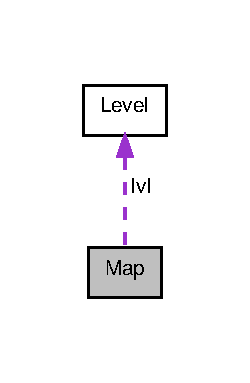
\includegraphics[width=120pt]{struct_map__coll__graph}
\end{center}
\end{figure}
\subsubsection*{Data Fields}
\begin{DoxyCompactItemize}
\item 
\hyperlink{struct_level}{Level} $\ast$ \hyperlink{struct_map_abca19b7de8e60347a507d1aeff95c764}{lvl}
\item 
int \hyperlink{struct_map_aa83bbdf2603e42824cd0bab44bf315c2}{x\-Scroll}
\item 
int \hyperlink{struct_map_ae50cb92a78d9e0a4f4bd718fc02bd294}{screen\-Width}
\item 
int \hyperlink{struct_map_a9ebc1dbd77788c4bfa27758a6725413f}{screen\-Height}
\end{DoxyCompactItemize}


\subsubsection{Detailed Description}
The map structure 

\subsubsection{Field Documentation}
\hypertarget{struct_map_abca19b7de8e60347a507d1aeff95c764}{\index{Map@{Map}!lvl@{lvl}}
\index{lvl@{lvl}!Map@{Map}}
\paragraph[{lvl}]{\setlength{\rightskip}{0pt plus 5cm}{\bf Level}$\ast$ lvl}}\label{struct_map_abca19b7de8e60347a507d1aeff95c764}
The level \hypertarget{struct_map_a9ebc1dbd77788c4bfa27758a6725413f}{\index{Map@{Map}!screen\-Height@{screen\-Height}}
\index{screen\-Height@{screen\-Height}!Map@{Map}}
\paragraph[{screen\-Height}]{\setlength{\rightskip}{0pt plus 5cm}int screen\-Height}}\label{struct_map_a9ebc1dbd77788c4bfa27758a6725413f}
The screen height \hypertarget{struct_map_ae50cb92a78d9e0a4f4bd718fc02bd294}{\index{Map@{Map}!screen\-Width@{screen\-Width}}
\index{screen\-Width@{screen\-Width}!Map@{Map}}
\paragraph[{screen\-Width}]{\setlength{\rightskip}{0pt plus 5cm}int screen\-Width}}\label{struct_map_ae50cb92a78d9e0a4f4bd718fc02bd294}
The Screen width \hypertarget{struct_map_aa83bbdf2603e42824cd0bab44bf315c2}{\index{Map@{Map}!x\-Scroll@{x\-Scroll}}
\index{x\-Scroll@{x\-Scroll}!Map@{Map}}
\paragraph[{x\-Scroll}]{\setlength{\rightskip}{0pt plus 5cm}int x\-Scroll}}\label{struct_map_aa83bbdf2603e42824cd0bab44bf315c2}
The xscroll 

The documentation for this struct was generated from the following file\-:\begin{DoxyCompactItemize}
\item 
\hyperlink{const_8h}{const.\-h}\end{DoxyCompactItemize}

\hypertarget{struct_sound}{\subsection{Sound Struct Reference}
\label{struct_sound}\index{Sound@{Sound}}
}


{\ttfamily \#include $<$sound.\-h$>$}

\subsubsection*{Data Fields}
\begin{DoxyCompactItemize}
\item 
\hypertarget{struct_sound_ae043bb23ee313709e1c605dd6c06d317}{F\-M\-O\-D\-\_\-\-S\-Y\-S\-T\-E\-M $\ast$ {\bfseries sys}}\label{struct_sound_ae043bb23ee313709e1c605dd6c06d317}

\item 
F\-M\-O\-D\-\_\-\-C\-H\-A\-N\-N\-E\-L $\ast$ \hyperlink{struct_sound_acca26c408c6140c8cdc0d8f49d31ad4a}{music}
\item 
F\-M\-O\-D\-\_\-\-C\-H\-A\-N\-N\-E\-L $\ast$ \hyperlink{struct_sound_a259d72174e26b5bb58146484cd54c1c8}{fx}
\item 
F\-M\-O\-D\-\_\-\-S\-O\-U\-N\-D $\ast$ \hyperlink{struct_sound_a1051e4654836160d314f8d49fe85ae77}{msc\-Sound}
\item 
F\-M\-O\-D\-\_\-\-S\-O\-U\-N\-D $\ast$ \hyperlink{struct_sound_a38b0d95773369da732eb81a289b52940}{fx\-Sound}
\item 
float \hyperlink{struct_sound_a6f06b572245c72c79f052b7efb89dc3b}{music\-Volume}
\item 
float \hyperlink{struct_sound_aedb4246a8bbae1c53f2f29572674b054}{fx\-Volume}
\end{DoxyCompactItemize}


\subsubsection{Detailed Description}
the sound gestion structure 

\subsubsection{Field Documentation}
\hypertarget{struct_sound_a259d72174e26b5bb58146484cd54c1c8}{\index{Sound@{Sound}!fx@{fx}}
\index{fx@{fx}!Sound@{Sound}}
\paragraph[{fx}]{\setlength{\rightskip}{0pt plus 5cm}F\-M\-O\-D\-\_\-\-C\-H\-A\-N\-N\-E\-L$\ast$ fx}}\label{struct_sound_a259d72174e26b5bb58146484cd54c1c8}
the music channel \hypertarget{struct_sound_a38b0d95773369da732eb81a289b52940}{\index{Sound@{Sound}!fx\-Sound@{fx\-Sound}}
\index{fx\-Sound@{fx\-Sound}!Sound@{Sound}}
\paragraph[{fx\-Sound}]{\setlength{\rightskip}{0pt plus 5cm}F\-M\-O\-D\-\_\-\-S\-O\-U\-N\-D$\ast$ fx\-Sound}}\label{struct_sound_a38b0d95773369da732eb81a289b52940}
the music sound \hypertarget{struct_sound_aedb4246a8bbae1c53f2f29572674b054}{\index{Sound@{Sound}!fx\-Volume@{fx\-Volume}}
\index{fx\-Volume@{fx\-Volume}!Sound@{Sound}}
\paragraph[{fx\-Volume}]{\setlength{\rightskip}{0pt plus 5cm}float fx\-Volume}}\label{struct_sound_aedb4246a8bbae1c53f2f29572674b054}
the music volume \hypertarget{struct_sound_a1051e4654836160d314f8d49fe85ae77}{\index{Sound@{Sound}!msc\-Sound@{msc\-Sound}}
\index{msc\-Sound@{msc\-Sound}!Sound@{Sound}}
\paragraph[{msc\-Sound}]{\setlength{\rightskip}{0pt plus 5cm}F\-M\-O\-D\-\_\-\-S\-O\-U\-N\-D$\ast$ msc\-Sound}}\label{struct_sound_a1051e4654836160d314f8d49fe85ae77}
the effects channel \hypertarget{struct_sound_acca26c408c6140c8cdc0d8f49d31ad4a}{\index{Sound@{Sound}!music@{music}}
\index{music@{music}!Sound@{Sound}}
\paragraph[{music}]{\setlength{\rightskip}{0pt plus 5cm}F\-M\-O\-D\-\_\-\-C\-H\-A\-N\-N\-E\-L$\ast$ music}}\label{struct_sound_acca26c408c6140c8cdc0d8f49d31ad4a}
the sound system \hypertarget{struct_sound_a6f06b572245c72c79f052b7efb89dc3b}{\index{Sound@{Sound}!music\-Volume@{music\-Volume}}
\index{music\-Volume@{music\-Volume}!Sound@{Sound}}
\paragraph[{music\-Volume}]{\setlength{\rightskip}{0pt plus 5cm}float music\-Volume}}\label{struct_sound_a6f06b572245c72c79f052b7efb89dc3b}
the effects sound 

The documentation for this struct was generated from the following file\-:\begin{DoxyCompactItemize}
\item 
\hyperlink{sound_8h}{sound.\-h}\end{DoxyCompactItemize}

\chapter{File Documentation}
\hypertarget{const_8h}{\section{const.\-h File Reference}
\label{const_8h}\index{const.\-h@{const.\-h}}
}


contient les constantes du programme  


This graph shows which files directly or indirectly include this file\-:\nopagebreak
\begin{figure}[H]
\begin{center}
\leavevmode
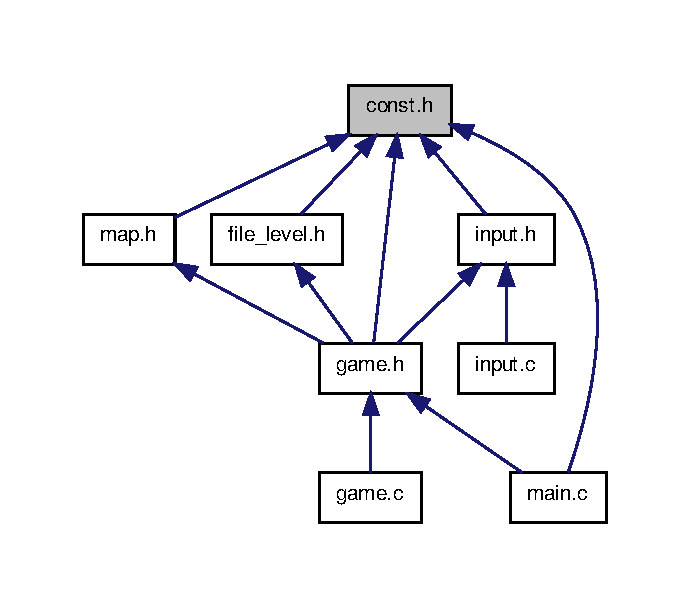
\includegraphics[width=350pt]{const_8h__dep__incl}
\end{center}
\end{figure}
\subsection*{Data Structures}
\begin{DoxyCompactItemize}
\item 
struct \hyperlink{struct_level}{Level}
\item 
struct \hyperlink{struct_map}{Map}
\end{DoxyCompactItemize}
\subsection*{Macros}
\begin{DoxyCompactItemize}
\item 
\hypertarget{const_8h_abad9ad5ae94fd56569e71c156349030b}{\#define {\bfseries T\-A\-I\-L\-L\-E\-\_\-\-B\-L\-O\-C}~16}\label{const_8h_abad9ad5ae94fd56569e71c156349030b}

\item 
\hypertarget{const_8h_a5b621c07985e98b04fc2d2195b85ad69}{\#define {\bfseries N\-B\-\_\-\-B\-L\-O\-C\-S\-\_\-\-L\-A\-R\-G\-E\-U\-R}~60}\label{const_8h_a5b621c07985e98b04fc2d2195b85ad69}

\item 
\hypertarget{const_8h_ad0de8de53b10369f89648fed34ce16c9}{\#define {\bfseries N\-B\-\_\-\-B\-L\-O\-C\-S\-\_\-\-H\-A\-U\-T\-E\-U\-R}~33}\label{const_8h_ad0de8de53b10369f89648fed34ce16c9}

\item 
\hypertarget{const_8h_a6068a247ff9ece1b0a9773c58144906c}{\#define {\bfseries L\-A\-R\-G\-E\-U\-R\-\_\-\-F\-E\-N\-E\-T\-R\-E}~T\-A\-I\-L\-L\-E\-\_\-\-B\-L\-O\-C $\ast$ N\-B\-\_\-\-B\-L\-O\-C\-S\-\_\-\-L\-A\-R\-G\-E\-U\-R}\label{const_8h_a6068a247ff9ece1b0a9773c58144906c}

\item 
\hypertarget{const_8h_afd1a1e285af564b849b17498e82e1a41}{\#define {\bfseries H\-A\-U\-T\-E\-U\-R\-\_\-\-F\-E\-N\-E\-T\-R\-E}~T\-A\-I\-L\-L\-E\-\_\-\-B\-L\-O\-C $\ast$ N\-B\-\_\-\-B\-L\-O\-C\-S\-\_\-\-H\-A\-U\-T\-E\-U\-R}\label{const_8h_afd1a1e285af564b849b17498e82e1a41}

\item 
\hypertarget{const_8h_ac92ca5ab87034a348decad7ee8d4bd1b}{\#define {\bfseries F\-P\-S}~60}\label{const_8h_ac92ca5ab87034a348decad7ee8d4bd1b}

\item 
\hypertarget{const_8h_a26141a4793db30295b597c3af901ddc8}{\#define {\bfseries T\-A\-I\-L\-L\-E\-\_\-\-M\-A\-X\-\_\-\-N\-O\-M\-\_\-\-F\-I\-C\-H\-I\-E\-R}~100}\label{const_8h_a26141a4793db30295b597c3af901ddc8}

\item 
\hypertarget{const_8h_a4295bab46a8fdcf8ff2106b2c32f15ad}{\#define {\bfseries T\-A\-I\-L\-L\-E\-\_\-\-S\-A\-U\-T}~17}\label{const_8h_a4295bab46a8fdcf8ff2106b2c32f15ad}

\item 
\hypertarget{const_8h_afe523953f60b9d8b73d97c8c673ef884}{\#define {\bfseries M\-A\-R\-G\-E\-\_\-\-S\-C\-R\-O\-L\-L\-I\-N\-G}~2}\label{const_8h_afe523953f60b9d8b73d97c8c673ef884}

\item 
\hypertarget{const_8h_a848d259eb2345aaa73fdfaeffb59afbd}{\#define {\bfseries P\-O\-U\-R\-C\-E\-N\-T\-A\-G\-E\-\_\-\-D\-E\-P\-L\-A\-C\-E\-M\-E\-N\-T}~0}\label{const_8h_a848d259eb2345aaa73fdfaeffb59afbd}

\item 
\hypertarget{const_8h_a95addb9496c5772d6e7bc43eabb16d8b}{\#define {\bfseries T\-I\-L\-E\-\_\-\-M\-A\-X}~8}\label{const_8h_a95addb9496c5772d6e7bc43eabb16d8b}

\end{DoxyCompactItemize}
\subsection*{Enumerations}
\begin{DoxyCompactItemize}
\item 
enum \{ {\bfseries V\-O\-I\-D} =0, 
{\bfseries G\-R\-A\-S\-S1} =1, 
{\bfseries G\-R\-O\-U\-N\-D1} =2, 
{\bfseries G\-R\-E\-Y\-\_\-\-W\-A\-L\-L} =3
 \}
\item 
enum \{ {\bfseries R\-I\-G\-H\-T}, 
{\bfseries L\-E\-F\-T}, 
{\bfseries U\-P}, 
{\bfseries D\-O\-W\-N}
 \}
\end{DoxyCompactItemize}


\subsection{Detailed Description}
contient les constantes du programme \begin{DoxyAuthor}{Author}
Xavier C\-O\-P\-O\-N\-E\-T 
\end{DoxyAuthor}
\begin{DoxyDate}{Date}
2014-\/02-\/27 
\end{DoxyDate}

\hypertarget{file_8c}{\section{file.\-c File Reference}
\label{file_8c}\index{file.\-c@{file.\-c}}
}


file access functions  


{\ttfamily \#include \char`\"{}file.\-h\char`\"{}}\\*
Include dependency graph for file.\-c\-:\nopagebreak
\begin{figure}[H]
\begin{center}
\leavevmode
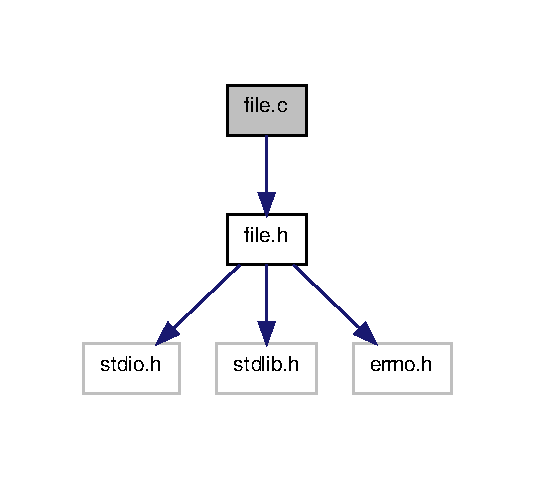
\includegraphics[width=256pt]{file_8c__incl}
\end{center}
\end{figure}
\subsection*{Functions}
\begin{DoxyCompactItemize}
\item 
F\-I\-L\-E $\ast$ \hyperlink{file_8c_ab763060cbdd57fdb704871d896fc492a}{open\-File} (char name\mbox{[}$\,$\mbox{]}, char mode\mbox{[}$\,$\mbox{]})
\item 
int \hyperlink{file_8c_adf55ac6bc5d81f94b54e4c8ea554f884}{close\-File} (F\-I\-L\-E $\ast$ptr\-\_\-file)
\end{DoxyCompactItemize}


\subsection{Detailed Description}
file access functions \begin{DoxyAuthor}{Author}
Remi B\-E\-R\-T\-H\-O 
\end{DoxyAuthor}
\begin{DoxyDate}{Date}
15/03/14 
\end{DoxyDate}


\subsection{Function Documentation}
\hypertarget{file_8c_adf55ac6bc5d81f94b54e4c8ea554f884}{\index{file.\-c@{file.\-c}!close\-File@{close\-File}}
\index{close\-File@{close\-File}!file.c@{file.\-c}}
\subsubsection[{close\-File}]{\setlength{\rightskip}{0pt plus 5cm}int close\-File (
\begin{DoxyParamCaption}
\item[{F\-I\-L\-E $\ast$}]{ptr\-\_\-file}
\end{DoxyParamCaption}
)}}\label{file_8c_adf55ac6bc5d81f94b54e4c8ea554f884}
close a file 
\begin{DoxyParams}[1]{Parameters}
\mbox{\tt in}  & {\em $\ast$ptr\-\_\-file} & the file to be closed \\
\hline
\end{DoxyParams}
\begin{DoxyReturn}{Returns}
int 0 if the file was succefuly closed, 1 if not 
\end{DoxyReturn}
\hypertarget{file_8c_ab763060cbdd57fdb704871d896fc492a}{\index{file.\-c@{file.\-c}!open\-File@{open\-File}}
\index{open\-File@{open\-File}!file.c@{file.\-c}}
\subsubsection[{open\-File}]{\setlength{\rightskip}{0pt plus 5cm}F\-I\-L\-E $\ast$ open\-File (
\begin{DoxyParamCaption}
\item[{char}]{name\mbox{[}$\,$\mbox{]}, }
\item[{char}]{mode\mbox{[}$\,$\mbox{]}}
\end{DoxyParamCaption}
)}}\label{file_8c_ab763060cbdd57fdb704871d896fc492a}
open a file 
\begin{DoxyParams}[1]{Parameters}
\mbox{\tt in}  & {\em name} & the file name/path \\
\hline
\mbox{\tt in}  & {\em mode} & the opening mode \\
\hline
\end{DoxyParams}
\begin{DoxyReturn}{Returns}
a pointer on the opened file, N\-U\-L\-L if error 
\end{DoxyReturn}

\hypertarget{file_8h}{\subsection{file.\-h File Reference}
\label{file_8h}\index{file.\-h@{file.\-h}}
}


\hyperlink{file_8c}{file.\-c} header  


{\ttfamily \#include $<$stdio.\-h$>$}\\*
{\ttfamily \#include $<$stdlib.\-h$>$}\\*
{\ttfamily \#include $<$errno.\-h$>$}\\*
\subsubsection*{Functions}
\begin{DoxyCompactItemize}
\item 
F\-I\-L\-E $\ast$ \hyperlink{file_8h_ae6218cf222b5ca17dce1ad7eb75346a9}{open\-File} (char nome\mbox{[}$\,$\mbox{]}, char mode\mbox{[}$\,$\mbox{]})
\item 
int \hyperlink{file_8h_a0fca34d72624f611d2cbeac47279bb1f}{close\-File} (F\-I\-L\-E $\ast$ptr\-\_\-fichier)
\end{DoxyCompactItemize}


\subsubsection{Detailed Description}
\hyperlink{file_8c}{file.\-c} header \begin{DoxyAuthor}{Author}
Remi B\-E\-R\-T\-H\-O, Glenn H\-E\-R\-R\-O\-U 
\end{DoxyAuthor}
\begin{DoxyDate}{Date}
2014-\/05-\/12 
\end{DoxyDate}


\subsubsection{Function Documentation}
\hypertarget{file_8h_a0fca34d72624f611d2cbeac47279bb1f}{\index{file.\-h@{file.\-h}!close\-File@{close\-File}}
\index{close\-File@{close\-File}!file.h@{file.\-h}}
\paragraph[{close\-File}]{\setlength{\rightskip}{0pt plus 5cm}int close\-File (
\begin{DoxyParamCaption}
\item[{F\-I\-L\-E $\ast$}]{ptr\-\_\-file}
\end{DoxyParamCaption}
)}}\label{file_8h_a0fca34d72624f611d2cbeac47279bb1f}
Close the given file 
\begin{DoxyParams}[1]{Parameters}
\mbox{\tt in}  & {\em $\ast$ptr\-\_\-file} & the file \\
\hline
\end{DoxyParams}
\begin{DoxyReturn}{Returns}
0 if the file has been succesfully closed, 1 otherwise 
\end{DoxyReturn}
\hypertarget{file_8h_ae6218cf222b5ca17dce1ad7eb75346a9}{\index{file.\-h@{file.\-h}!open\-File@{open\-File}}
\index{open\-File@{open\-File}!file.h@{file.\-h}}
\paragraph[{open\-File}]{\setlength{\rightskip}{0pt plus 5cm}F\-I\-L\-E$\ast$ open\-File (
\begin{DoxyParamCaption}
\item[{char}]{name\mbox{[}$\,$\mbox{]}, }
\item[{char}]{mode\mbox{[}$\,$\mbox{]}}
\end{DoxyParamCaption}
)}}\label{file_8h_ae6218cf222b5ca17dce1ad7eb75346a9}
Open a file which path is name with the given mode 
\begin{DoxyParams}[1]{Parameters}
\mbox{\tt in}  & {\em name\mbox{[}$\,$\mbox{]}} & name of the file \\
\hline
\mbox{\tt in}  & {\em mode\mbox{[}$\,$\mbox{]}} & the opening mode \\
\hline
\end{DoxyParams}
\begin{DoxyReturn}{Returns}
a pointer if the opening has been succesfull, N\-U\-L\-L otherwise 
\end{DoxyReturn}

\hypertarget{jeu_8c}{\section{jeu.\-c File Reference}
\label{jeu_8c}\index{jeu.\-c@{jeu.\-c}}
}


contient les fonction liées au jeu  


{\ttfamily \#include \char`\"{}jeu.\-h\char`\"{}}\\*
Include dependency graph for jeu.\-c\-:
\nopagebreak
\begin{figure}[H]
\begin{center}
\leavevmode
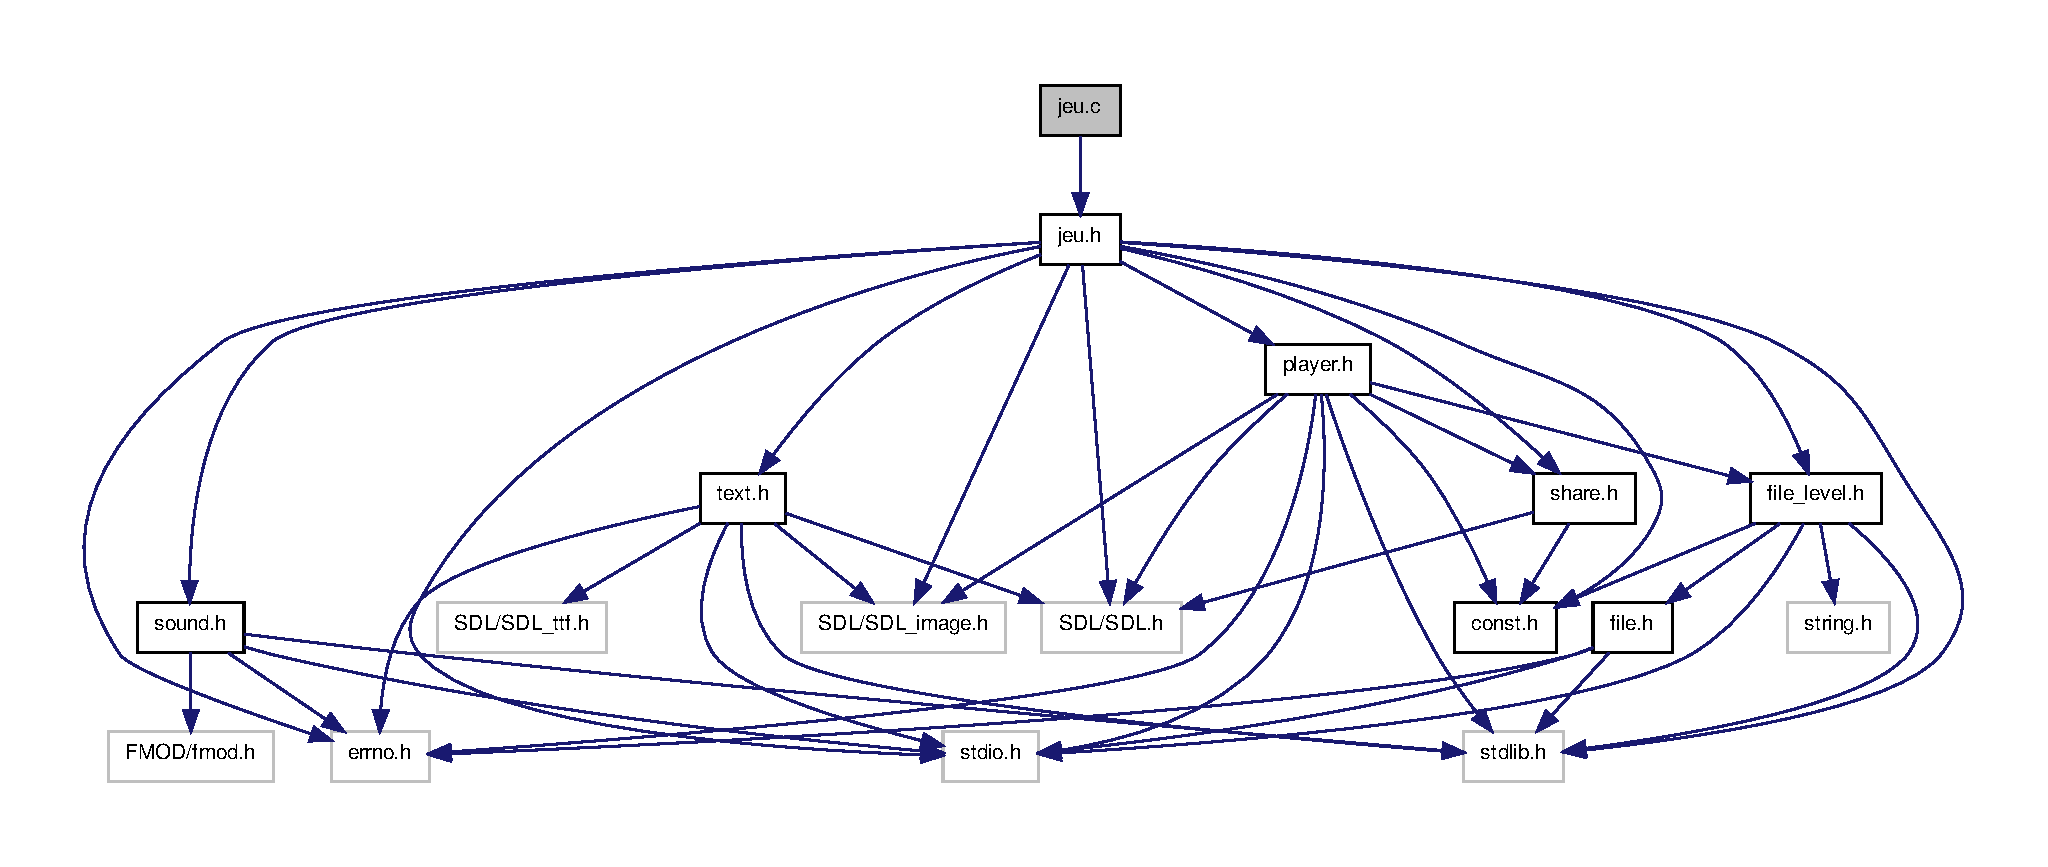
\includegraphics[width=350pt]{jeu_8c__incl}
\end{center}
\end{figure}
\subsection*{Functions}
\begin{DoxyCompactItemize}
\item 
void \hyperlink{jeu_8c_ae9a0a76fc32328b2b6e4923f01c7de89}{jouer} (S\-D\-L\-\_\-\-Surface $\ast$screen, char $\ast$level\-\_\-name)
\item 
\hypertarget{jeu_8c_a93e611e5879ce7399e92ab03d151acc3}{void {\bfseries update\-Screen\-Map} (S\-D\-L\-\_\-\-Surface $\ast$screen, \hyperlink{struct_map}{Map} $\ast$m)}\label{jeu_8c_a93e611e5879ce7399e92ab03d151acc3}

\item 
void \hyperlink{jeu_8c_a6f031e5ad35ada9038d3a72a56053760}{scrolling} (\hyperlink{struct_map}{Map} $\ast$m, int direction, float speed)
\item 
\hypertarget{jeu_8c_ad16d857230b785e820b9b497b50b7fff}{Uint32 {\bfseries decomptage} (Uint32 intervalle, void $\ast$parametre)}\label{jeu_8c_ad16d857230b785e820b9b497b50b7fff}

\item 
\hyperlink{struct_map}{Map} $\ast$ \hyperlink{jeu_8c_a49f0a1130f157d0c35bd28f892b6a76b}{init\-Map} (\hyperlink{struct_level}{Level} $\ast$lvl, S\-D\-L\-\_\-\-Surface $\ast$screen)
\item 
\hypertarget{jeu_8c_ac8d4dd6fc80c79d9cb5899684740d074}{void {\bfseries free\-Map} (\hyperlink{struct_map}{Map} $\ast$m)}\label{jeu_8c_ac8d4dd6fc80c79d9cb5899684740d074}

\item 
void \hyperlink{jeu_8c_a8c1653310113496aa24fa5d3c86461a6}{print\-Game\-Over} (S\-D\-L\-\_\-\-Surface $\ast$screen, int $\ast$continuer)
\item 
void \hyperlink{jeu_8c_a297ffd698dfe4680eb42f1a1335697c2}{move} (int move\-\_\-left, int move\-\_\-right, \hyperlink{struct_character}{Character} $\ast$player, \hyperlink{struct_map}{Map} $\ast$m, float speed)
\end{DoxyCompactItemize}


\subsection{Detailed Description}
contient les fonction liées au jeu \begin{DoxyAuthor}{Author}
Xavier C\-O\-P\-O\-N\-E\-T 
\end{DoxyAuthor}
\begin{DoxyDate}{Date}
2014-\/02-\/27 
\end{DoxyDate}


\subsection{Function Documentation}
\hypertarget{jeu_8c_a49f0a1130f157d0c35bd28f892b6a76b}{\index{jeu.\-c@{jeu.\-c}!init\-Map@{init\-Map}}
\index{init\-Map@{init\-Map}!jeu.c@{jeu.\-c}}
\subsubsection[{init\-Map}]{\setlength{\rightskip}{0pt plus 5cm}{\bf Map} $\ast$ init\-Map (
\begin{DoxyParamCaption}
\item[{{\bf Level} $\ast$}]{lvl, }
\item[{S\-D\-L\-\_\-\-Surface $\ast$}]{screen}
\end{DoxyParamCaption}
)}}\label{jeu_8c_a49f0a1130f157d0c35bd28f892b6a76b}
initialise la carte 
\begin{DoxyParams}[1]{Parameters}
\mbox{\tt in}  & {\em screen} & l'écran de jeu \\
\hline
\mbox{\tt in}  & {\em level} & le niveau \\
\hline
\end{DoxyParams}
\begin{DoxyReturn}{Returns}
un pointeur sur la carte initialisée 
\end{DoxyReturn}
\hypertarget{jeu_8c_ae9a0a76fc32328b2b6e4923f01c7de89}{\index{jeu.\-c@{jeu.\-c}!jouer@{jouer}}
\index{jouer@{jouer}!jeu.c@{jeu.\-c}}
\subsubsection[{jouer}]{\setlength{\rightskip}{0pt plus 5cm}void jouer (
\begin{DoxyParamCaption}
\item[{S\-D\-L\-\_\-\-Surface $\ast$}]{screen, }
\item[{char $\ast$}]{level\-\_\-name}
\end{DoxyParamCaption}
)}}\label{jeu_8c_ae9a0a76fc32328b2b6e4923f01c7de89}
contient la boucle principale du jeu qui appelle les fonctions 
\begin{DoxyParams}[1]{Parameters}
\mbox{\tt in,out}  & {\em screen} & L'écran de jeu \\
\hline
\mbox{\tt in}  & {\em lvel\-\_\-name} & le nom du niveau \\
\hline
\end{DoxyParams}


Here is the call graph for this function\-:\nopagebreak
\begin{figure}[H]
\begin{center}
\leavevmode
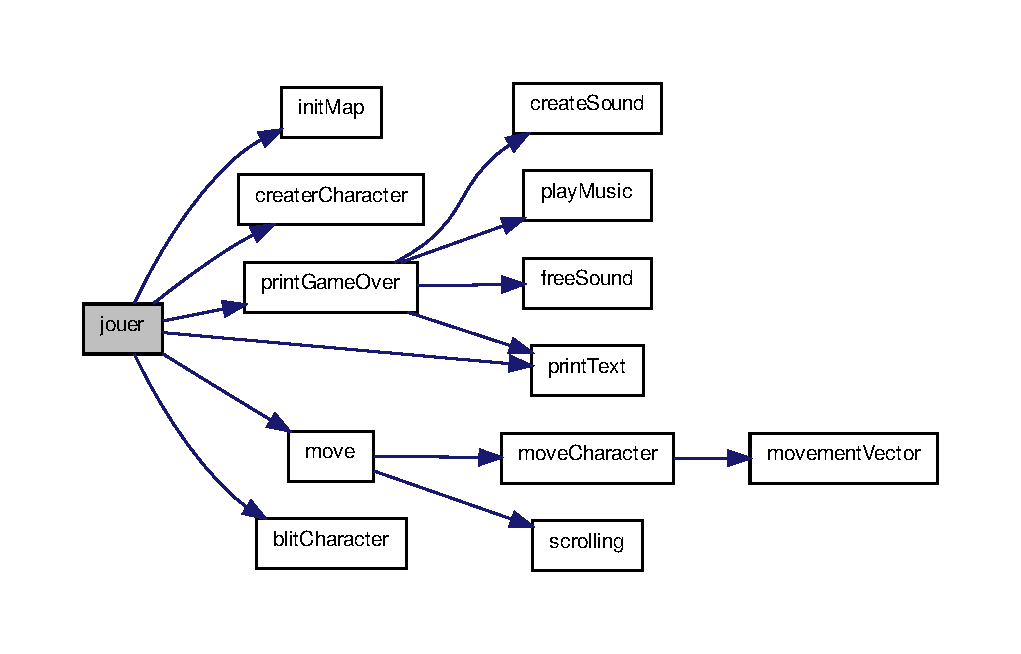
\includegraphics[width=350pt]{jeu_8c_ae9a0a76fc32328b2b6e4923f01c7de89_cgraph}
\end{center}
\end{figure}


\hypertarget{jeu_8c_a297ffd698dfe4680eb42f1a1335697c2}{\index{jeu.\-c@{jeu.\-c}!move@{move}}
\index{move@{move}!jeu.c@{jeu.\-c}}
\subsubsection[{move}]{\setlength{\rightskip}{0pt plus 5cm}void move (
\begin{DoxyParamCaption}
\item[{int}]{move\-\_\-left, }
\item[{int}]{move\-\_\-right, }
\item[{{\bf Character} $\ast$}]{player, }
\item[{{\bf Map} $\ast$}]{m, }
\item[{float}]{speed}
\end{DoxyParamCaption}
)}}\label{jeu_8c_a297ffd698dfe4680eb42f1a1335697c2}
Deplace le joueur et scrolle l'ecran si besoin 
\begin{DoxyParams}[1]{Parameters}
\mbox{\tt in}  & {\em move\-\_\-left} & booleen pour savoir si l'on bouge a gauche \\
\hline
\mbox{\tt in}  & {\em move\-\_\-right} & booleen pour savoir si l'on bouge a droite \\
\hline
\mbox{\tt in}  & {\em player} & le joueur \\
\hline
\mbox{\tt in}  & {\em m} & la carte \\
\hline
\end{DoxyParams}


Here is the call graph for this function\-:\nopagebreak
\begin{figure}[H]
\begin{center}
\leavevmode
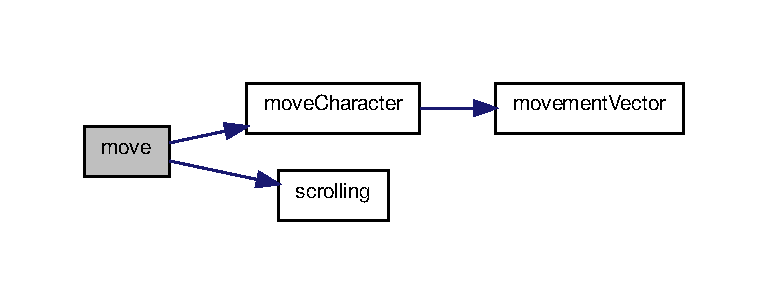
\includegraphics[width=350pt]{jeu_8c_a297ffd698dfe4680eb42f1a1335697c2_cgraph}
\end{center}
\end{figure}


\hypertarget{jeu_8c_a8c1653310113496aa24fa5d3c86461a6}{\index{jeu.\-c@{jeu.\-c}!print\-Game\-Over@{print\-Game\-Over}}
\index{print\-Game\-Over@{print\-Game\-Over}!jeu.c@{jeu.\-c}}
\subsubsection[{print\-Game\-Over}]{\setlength{\rightskip}{0pt plus 5cm}void print\-Game\-Over (
\begin{DoxyParamCaption}
\item[{S\-D\-L\-\_\-\-Surface $\ast$}]{screen, }
\item[{int $\ast$}]{continuer}
\end{DoxyParamCaption}
)}}\label{jeu_8c_a8c1653310113496aa24fa5d3c86461a6}
affiche le message de game overflow\-\_\-error 
\begin{DoxyParams}[1]{Parameters}
\mbox{\tt out}  & {\em screen} & l'écran de jeu \\
\hline
\end{DoxyParams}


Here is the call graph for this function\-:\nopagebreak
\begin{figure}[H]
\begin{center}
\leavevmode
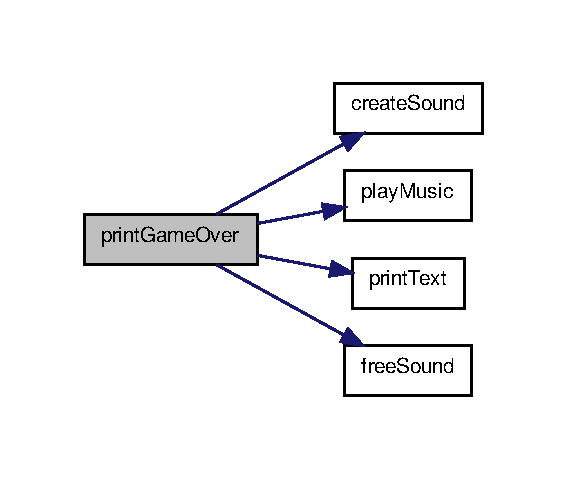
\includegraphics[width=272pt]{jeu_8c_a8c1653310113496aa24fa5d3c86461a6_cgraph}
\end{center}
\end{figure}


\hypertarget{jeu_8c_a6f031e5ad35ada9038d3a72a56053760}{\index{jeu.\-c@{jeu.\-c}!scrolling@{scrolling}}
\index{scrolling@{scrolling}!jeu.c@{jeu.\-c}}
\subsubsection[{scrolling}]{\setlength{\rightskip}{0pt plus 5cm}void scrolling (
\begin{DoxyParamCaption}
\item[{{\bf Map} $\ast$}]{m, }
\item[{int}]{direction, }
\item[{float}]{speed}
\end{DoxyParamCaption}
)}}\label{jeu_8c_a6f031e5ad35ada9038d3a72a56053760}
effectue un scrolling 
\begin{DoxyParams}[1]{Parameters}
\mbox{\tt in,out}  & {\em map} & Le niveau à gérer \\
\hline
\mbox{\tt in}  & {\em direction} & La direction de scrolling \\
\hline
\mbox{\tt in}  & {\em speed} & la vitesse de scrolling \\
\hline
\end{DoxyParams}

\hypertarget{jeu_8h}{\section{jeu.\-h File Reference}
\label{jeu_8h}\index{jeu.\-h@{jeu.\-h}}
}


header de \hyperlink{jeu_8c}{jeu.\-c}  


{\ttfamily \#include $<$stdlib.\-h$>$}\\*
{\ttfamily \#include $<$stdio.\-h$>$}\\*
{\ttfamily \#include $<$errno.\-h$>$}\\*
{\ttfamily \#include $<$S\-D\-L/\-S\-D\-L.\-h$>$}\\*
{\ttfamily \#include $<$S\-D\-L/\-S\-D\-L\-\_\-image.\-h$>$}\\*
{\ttfamily \#include \char`\"{}const.\-h\char`\"{}}\\*
{\ttfamily \#include \char`\"{}text.\-h\char`\"{}}\\*
{\ttfamily \#include \char`\"{}sound.\-h\char`\"{}}\\*
{\ttfamily \#include \char`\"{}share.\-h\char`\"{}}\\*
{\ttfamily \#include \char`\"{}player.\-h\char`\"{}}\\*
{\ttfamily \#include \char`\"{}file\-\_\-level.\-h\char`\"{}}\\*
Include dependency graph for jeu.\-h\-:
\nopagebreak
\begin{figure}[H]
\begin{center}
\leavevmode
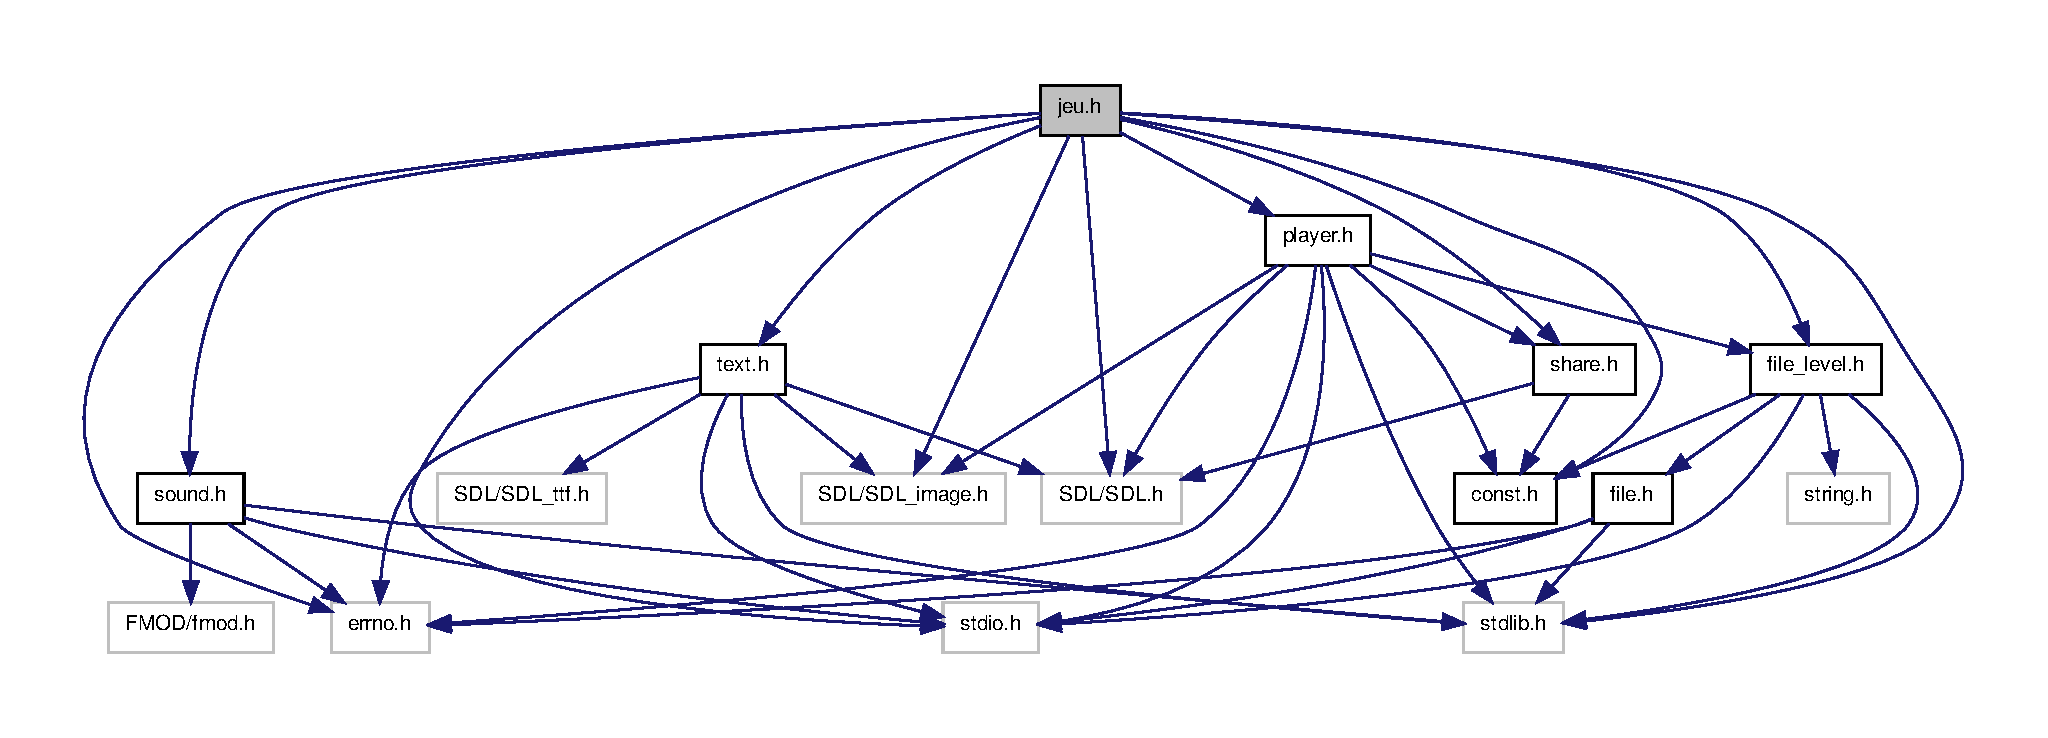
\includegraphics[width=350pt]{jeu_8h__incl}
\end{center}
\end{figure}
This graph shows which files directly or indirectly include this file\-:
\nopagebreak
\begin{figure}[H]
\begin{center}
\leavevmode
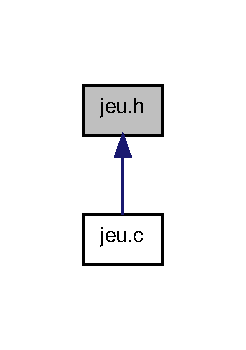
\includegraphics[width=118pt]{jeu_8h__dep__incl}
\end{center}
\end{figure}
\subsection*{Macros}
\begin{DoxyCompactItemize}
\item 
\hypertarget{jeu_8h_a848d259eb2345aaa73fdfaeffb59afbd}{\#define {\bfseries P\-O\-U\-R\-C\-E\-N\-T\-A\-G\-E\-\_\-\-D\-E\-P\-L\-A\-C\-E\-M\-E\-N\-T}~15}\label{jeu_8h_a848d259eb2345aaa73fdfaeffb59afbd}

\end{DoxyCompactItemize}
\subsection*{Functions}
\begin{DoxyCompactItemize}
\item 
void \hyperlink{jeu_8h_ae9a0a76fc32328b2b6e4923f01c7de89}{jouer} (S\-D\-L\-\_\-\-Surface $\ast$screen, char $\ast$level\-\_\-name)
\item 
\hypertarget{jeu_8h_a93e611e5879ce7399e92ab03d151acc3}{void {\bfseries update\-Screen\-Map} (S\-D\-L\-\_\-\-Surface $\ast$screen, \hyperlink{struct_map}{Map} $\ast$m)}\label{jeu_8h_a93e611e5879ce7399e92ab03d151acc3}

\item 
void \hyperlink{jeu_8h_a6f031e5ad35ada9038d3a72a56053760}{scrolling} (\hyperlink{struct_map}{Map} $\ast$m, int direction, float speed)
\item 
\hypertarget{jeu_8h_ad16d857230b785e820b9b497b50b7fff}{Uint32 {\bfseries decomptage} (Uint32 intervalle, void $\ast$parametre)}\label{jeu_8h_ad16d857230b785e820b9b497b50b7fff}

\item 
\hyperlink{struct_map}{Map} $\ast$ \hyperlink{jeu_8h_a7ab71b3daf19eb6c3b544d408b8826e0}{init\-Map} (\hyperlink{struct_level}{Level} $\ast$lvl, S\-D\-L\-\_\-\-Surface $\ast$screen)
\item 
\hypertarget{jeu_8h_ac8d4dd6fc80c79d9cb5899684740d074}{void {\bfseries free\-Map} (\hyperlink{struct_map}{Map} $\ast$m)}\label{jeu_8h_ac8d4dd6fc80c79d9cb5899684740d074}

\item 
void \hyperlink{jeu_8h_a8c1653310113496aa24fa5d3c86461a6}{print\-Game\-Over} (S\-D\-L\-\_\-\-Surface $\ast$screen, int $\ast$continuer)
\item 
void \hyperlink{jeu_8h_a297ffd698dfe4680eb42f1a1335697c2}{move} (int move\-\_\-left, int move\-\_\-right, \hyperlink{struct_character}{Character} $\ast$player, \hyperlink{struct_map}{Map} $\ast$m, float speed)
\end{DoxyCompactItemize}


\subsection{Detailed Description}
header de \hyperlink{jeu_8c}{jeu.\-c} \begin{DoxyAuthor}{Author}
Xavier C\-O\-P\-O\-N\-E\-T 
\end{DoxyAuthor}
\begin{DoxyDate}{Date}
2014-\/02-\/27 
\end{DoxyDate}


\subsection{Function Documentation}
\hypertarget{jeu_8h_a7ab71b3daf19eb6c3b544d408b8826e0}{\index{jeu.\-h@{jeu.\-h}!init\-Map@{init\-Map}}
\index{init\-Map@{init\-Map}!jeu.h@{jeu.\-h}}
\subsubsection[{init\-Map}]{\setlength{\rightskip}{0pt plus 5cm}{\bf Map}$\ast$ init\-Map (
\begin{DoxyParamCaption}
\item[{{\bf Level} $\ast$}]{lvl, }
\item[{S\-D\-L\-\_\-\-Surface $\ast$}]{screen}
\end{DoxyParamCaption}
)}}\label{jeu_8h_a7ab71b3daf19eb6c3b544d408b8826e0}
initialise la carte 
\begin{DoxyParams}[1]{Parameters}
\mbox{\tt in}  & {\em screen} & l'écran de jeu \\
\hline
\mbox{\tt in}  & {\em level} & le niveau \\
\hline
\end{DoxyParams}
\begin{DoxyReturn}{Returns}
un pointeur sur la carte initialisée 
\end{DoxyReturn}
\hypertarget{jeu_8h_ae9a0a76fc32328b2b6e4923f01c7de89}{\index{jeu.\-h@{jeu.\-h}!jouer@{jouer}}
\index{jouer@{jouer}!jeu.h@{jeu.\-h}}
\subsubsection[{jouer}]{\setlength{\rightskip}{0pt plus 5cm}void jouer (
\begin{DoxyParamCaption}
\item[{S\-D\-L\-\_\-\-Surface $\ast$}]{screen, }
\item[{char $\ast$}]{level\-\_\-name}
\end{DoxyParamCaption}
)}}\label{jeu_8h_ae9a0a76fc32328b2b6e4923f01c7de89}
contient la boucle principale du jeu qui appelle les fonctions 
\begin{DoxyParams}[1]{Parameters}
\mbox{\tt in,out}  & {\em screen} & L'écran de jeu \\
\hline
\mbox{\tt in}  & {\em lvel\-\_\-name} & le nom du niveau \\
\hline
\end{DoxyParams}


Here is the call graph for this function\-:\nopagebreak
\begin{figure}[H]
\begin{center}
\leavevmode
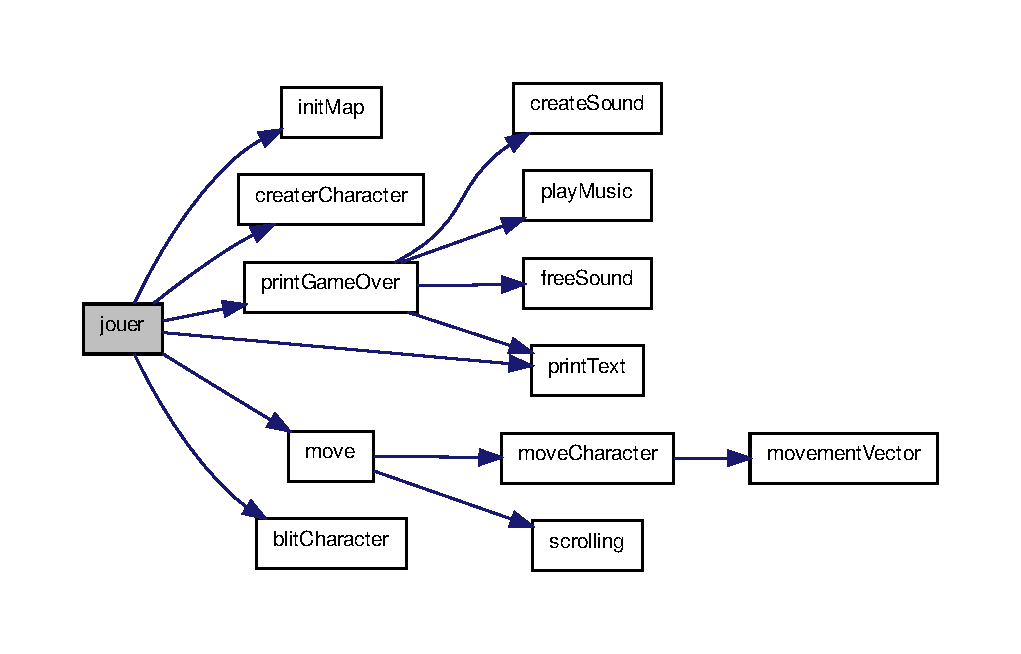
\includegraphics[width=350pt]{jeu_8h_ae9a0a76fc32328b2b6e4923f01c7de89_cgraph}
\end{center}
\end{figure}


\hypertarget{jeu_8h_a297ffd698dfe4680eb42f1a1335697c2}{\index{jeu.\-h@{jeu.\-h}!move@{move}}
\index{move@{move}!jeu.h@{jeu.\-h}}
\subsubsection[{move}]{\setlength{\rightskip}{0pt plus 5cm}void move (
\begin{DoxyParamCaption}
\item[{int}]{move\-\_\-left, }
\item[{int}]{move\-\_\-right, }
\item[{{\bf Character} $\ast$}]{player, }
\item[{{\bf Map} $\ast$}]{m, }
\item[{float}]{speed}
\end{DoxyParamCaption}
)}}\label{jeu_8h_a297ffd698dfe4680eb42f1a1335697c2}
Deplace le joueur et scrolle l'ecran si besoin 
\begin{DoxyParams}[1]{Parameters}
\mbox{\tt in}  & {\em move\-\_\-left} & booleen pour savoir si l'on bouge a gauche \\
\hline
\mbox{\tt in}  & {\em move\-\_\-right} & booleen pour savoir si l'on bouge a droite \\
\hline
\mbox{\tt in}  & {\em player} & le joueur \\
\hline
\mbox{\tt in}  & {\em m} & la carte \\
\hline
\end{DoxyParams}


Here is the call graph for this function\-:\nopagebreak
\begin{figure}[H]
\begin{center}
\leavevmode
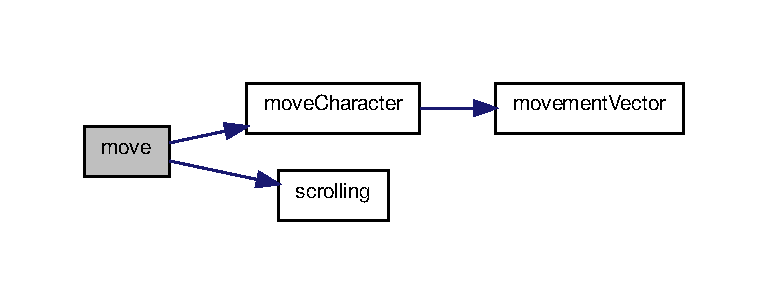
\includegraphics[width=350pt]{jeu_8h_a297ffd698dfe4680eb42f1a1335697c2_cgraph}
\end{center}
\end{figure}


\hypertarget{jeu_8h_a8c1653310113496aa24fa5d3c86461a6}{\index{jeu.\-h@{jeu.\-h}!print\-Game\-Over@{print\-Game\-Over}}
\index{print\-Game\-Over@{print\-Game\-Over}!jeu.h@{jeu.\-h}}
\subsubsection[{print\-Game\-Over}]{\setlength{\rightskip}{0pt plus 5cm}void print\-Game\-Over (
\begin{DoxyParamCaption}
\item[{S\-D\-L\-\_\-\-Surface $\ast$}]{screen, }
\item[{int $\ast$}]{continuer}
\end{DoxyParamCaption}
)}}\label{jeu_8h_a8c1653310113496aa24fa5d3c86461a6}
affiche le message de game overflow\-\_\-error 
\begin{DoxyParams}[1]{Parameters}
\mbox{\tt out}  & {\em screen} & l'écran de jeu \\
\hline
\end{DoxyParams}


Here is the call graph for this function\-:\nopagebreak
\begin{figure}[H]
\begin{center}
\leavevmode
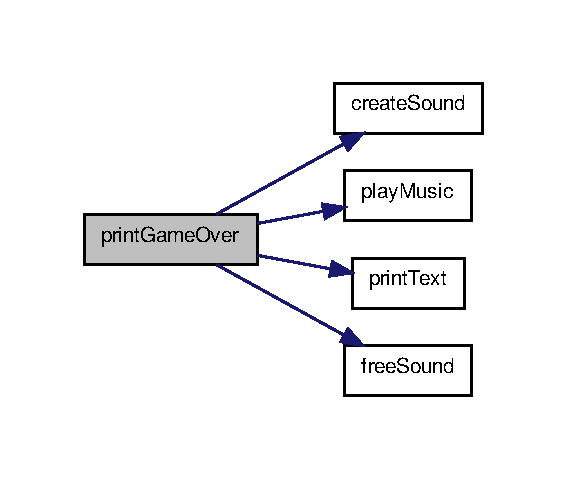
\includegraphics[width=272pt]{jeu_8h_a8c1653310113496aa24fa5d3c86461a6_cgraph}
\end{center}
\end{figure}


\hypertarget{jeu_8h_a6f031e5ad35ada9038d3a72a56053760}{\index{jeu.\-h@{jeu.\-h}!scrolling@{scrolling}}
\index{scrolling@{scrolling}!jeu.h@{jeu.\-h}}
\subsubsection[{scrolling}]{\setlength{\rightskip}{0pt plus 5cm}void scrolling (
\begin{DoxyParamCaption}
\item[{{\bf Map} $\ast$}]{m, }
\item[{int}]{direction, }
\item[{float}]{speed}
\end{DoxyParamCaption}
)}}\label{jeu_8h_a6f031e5ad35ada9038d3a72a56053760}
effectue un scrolling 
\begin{DoxyParams}[1]{Parameters}
\mbox{\tt in,out}  & {\em map} & Le niveau à gérer \\
\hline
\mbox{\tt in}  & {\em direction} & La direction de scrolling \\
\hline
\mbox{\tt in}  & {\em speed} & la vitesse de scrolling \\
\hline
\end{DoxyParams}

\hypertarget{menu_8c}{\subsection{menu.\-c File Reference}
\label{menu_8c}\index{menu.\-c@{menu.\-c}}
}


Contain the main menu management.  


{\ttfamily \#include \char`\"{}menu.\-h\char`\"{}}\\*
\subsubsection*{Functions}
\begin{DoxyCompactItemize}
\item 
int \hyperlink{menu_8c_a9b210afb32784dfdf07bd2d4ef25e0bc}{menu} (S\-D\-L\-\_\-\-Surface $\ast$screen, int $\ast$choice, int $\ast$go)
\item 
int \hyperlink{menu_8c_a2e385684b2e6cc22168f98525f3693d8}{menu\-Tile\-Set} (S\-D\-L\-\_\-\-Surface $\ast$screen, char tile\-Set\-\_\-name\mbox{[}\hyperlink{const_8h_a9620725a4f8ab39e0912adede7cb347f}{M\-A\-X\-\_\-\-L\-E\-N\-G\-T\-H\-\_\-\-F\-I\-L\-E\-\_\-\-N\-A\-M\-E}\mbox{]})
\end{DoxyCompactItemize}


\subsubsection{Detailed Description}
Contain the main menu management. \begin{DoxyAuthor}{Author}
Glenn H\-E\-R\-R\-O\-U 
\end{DoxyAuthor}
\begin{DoxyDate}{Date}
2014-\/04-\/20 
\end{DoxyDate}


\subsubsection{Function Documentation}
\hypertarget{menu_8c_a9b210afb32784dfdf07bd2d4ef25e0bc}{\index{menu.\-c@{menu.\-c}!menu@{menu}}
\index{menu@{menu}!menu.c@{menu.\-c}}
\paragraph[{menu}]{\setlength{\rightskip}{0pt plus 5cm}int menu (
\begin{DoxyParamCaption}
\item[{S\-D\-L\-\_\-\-Surface $\ast$}]{screen, }
\item[{int $\ast$}]{choice, }
\item[{int $\ast$}]{go}
\end{DoxyParamCaption}
)}}\label{menu_8c_a9b210afb32784dfdf07bd2d4ef25e0bc}
Display the menu on the screen 
\begin{DoxyParams}[1]{Parameters}
\mbox{\tt out}  & {\em screen} & the screen of the game \\
\hline
\mbox{\tt out}  & {\em choice} & the option selected \\
\hline
\mbox{\tt out}  & {\em go} & the main loop validation \\
\hline
\end{DoxyParams}
\begin{DoxyReturn}{Returns}
1 if an option has been selected 
\end{DoxyReturn}


Here is the call graph for this function\-:\nopagebreak
\begin{figure}[H]
\begin{center}
\leavevmode
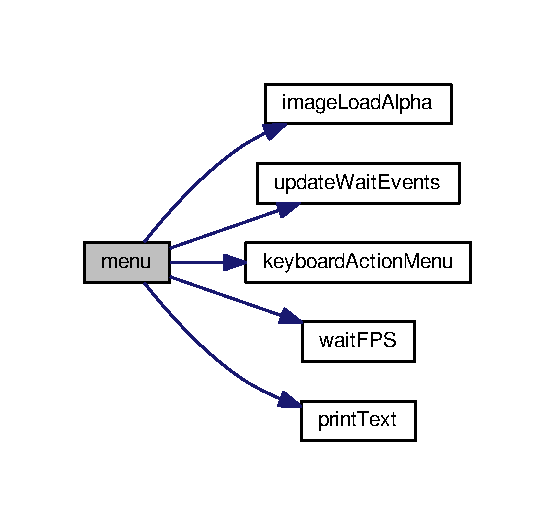
\includegraphics[width=266pt]{menu_8c_a9b210afb32784dfdf07bd2d4ef25e0bc_cgraph}
\end{center}
\end{figure}


\hypertarget{menu_8c_a2e385684b2e6cc22168f98525f3693d8}{\index{menu.\-c@{menu.\-c}!menu\-Tile\-Set@{menu\-Tile\-Set}}
\index{menu\-Tile\-Set@{menu\-Tile\-Set}!menu.c@{menu.\-c}}
\paragraph[{menu\-Tile\-Set}]{\setlength{\rightskip}{0pt plus 5cm}int menu\-Tile\-Set (
\begin{DoxyParamCaption}
\item[{S\-D\-L\-\_\-\-Surface $\ast$}]{screen, }
\item[{char}]{tile\-Set\-\_\-name\mbox{[}\-M\-A\-X\-\_\-\-L\-E\-N\-G\-T\-H\-\_\-\-F\-I\-L\-E\-\_\-\-N\-A\-M\-E\mbox{]}}
\end{DoxyParamCaption}
)}}\label{menu_8c_a2e385684b2e6cc22168f98525f3693d8}
Display the tileset menu on the screen 
\begin{DoxyParams}[1]{Parameters}
\mbox{\tt out}  & {\em screen} & the screen of the game \\
\hline
\mbox{\tt out}  & {\em tile\-Set\-\_\-name} & The name of the tile\-Set selected \\
\hline
\end{DoxyParams}
\begin{DoxyReturn}{Returns}
1 if a tileset has been selected 
\end{DoxyReturn}


Here is the call graph for this function\-:\nopagebreak
\begin{figure}[H]
\begin{center}
\leavevmode
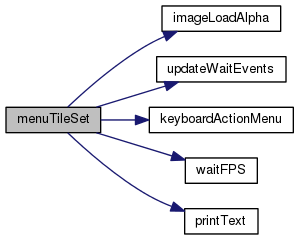
\includegraphics[width=296pt]{menu_8c_a2e385684b2e6cc22168f98525f3693d8_cgraph}
\end{center}
\end{figure}



\hypertarget{menu_8h}{\section{menu.\-h File Reference}
\label{menu_8h}\index{menu.\-h@{menu.\-h}}
}


header de \hyperlink{menu_8c}{menu.\-c}  


{\ttfamily \#include $<$stdlib.\-h$>$}\\*
{\ttfamily \#include $<$stdio.\-h$>$}\\*
{\ttfamily \#include $<$errno.\-h$>$}\\*
{\ttfamily \#include $<$S\-D\-L/\-S\-D\-L.\-h$>$}\\*
{\ttfamily \#include $<$S\-D\-L/\-S\-D\-L\-\_\-image.\-h$>$}\\*
{\ttfamily \#include $<$S\-D\-L/\-S\-D\-L\-\_\-ttf.\-h$>$}\\*
{\ttfamily \#include \char`\"{}const.\-h\char`\"{}}\\*
{\ttfamily \#include \char`\"{}text.\-h\char`\"{}}\\*
{\ttfamily \#include \char`\"{}sound.\-h\char`\"{}}\\*
{\ttfamily \#include \char`\"{}share.\-h\char`\"{}}\\*
Include dependency graph for menu.\-h\-:
\nopagebreak
\begin{figure}[H]
\begin{center}
\leavevmode
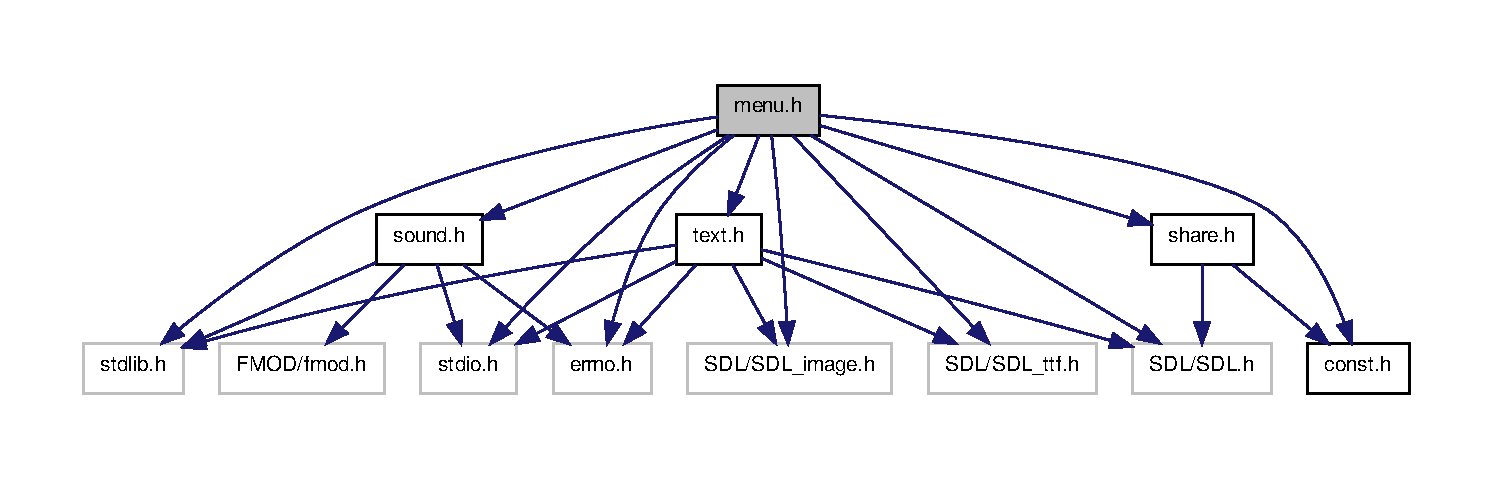
\includegraphics[width=350pt]{menu_8h__incl}
\end{center}
\end{figure}
This graph shows which files directly or indirectly include this file\-:
\nopagebreak
\begin{figure}[H]
\begin{center}
\leavevmode
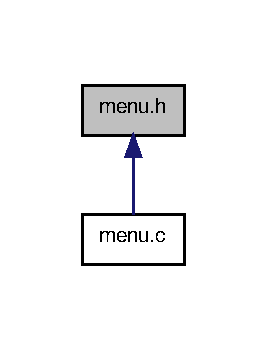
\includegraphics[width=128pt]{menu_8h__dep__incl}
\end{center}
\end{figure}
\subsection*{Functions}
\begin{DoxyCompactItemize}
\item 
\hypertarget{menu_8h_a4604196e3bcbd88eb0a7888effc9dc6f}{int {\bfseries menu} (S\-D\-L\-\_\-\-Surface $\ast$screen, int $\ast$continuer, \hyperlink{struct_sound}{Sound} $\ast$s)}\label{menu_8h_a4604196e3bcbd88eb0a7888effc9dc6f}

\item 
\hypertarget{menu_8h_a0943f574afa5b9e3928862fd99df0d4b}{Uint32 {\bfseries blink\-Text} (Uint32 intervalle, void $\ast$parametre)}\label{menu_8h_a0943f574afa5b9e3928862fd99df0d4b}

\end{DoxyCompactItemize}


\subsection{Detailed Description}
header de \hyperlink{menu_8c}{menu.\-c} \begin{DoxyAuthor}{Author}
Xavier C\-O\-P\-O\-N\-E\-T 
\end{DoxyAuthor}
\begin{DoxyDate}{Date}
2014-\/02-\/27 
\end{DoxyDate}

\hypertarget{menu__level_8c}{\section{menu\-\_\-level.\-c File Reference}
\label{menu__level_8c}\index{menu\-\_\-level.\-c@{menu\-\_\-level.\-c}}
}


level choose menu  


{\ttfamily \#include \char`\"{}menu\-\_\-level.\-h\char`\"{}}\\*
Include dependency graph for menu\-\_\-level.\-c\-:
\nopagebreak
\begin{figure}[H]
\begin{center}
\leavevmode
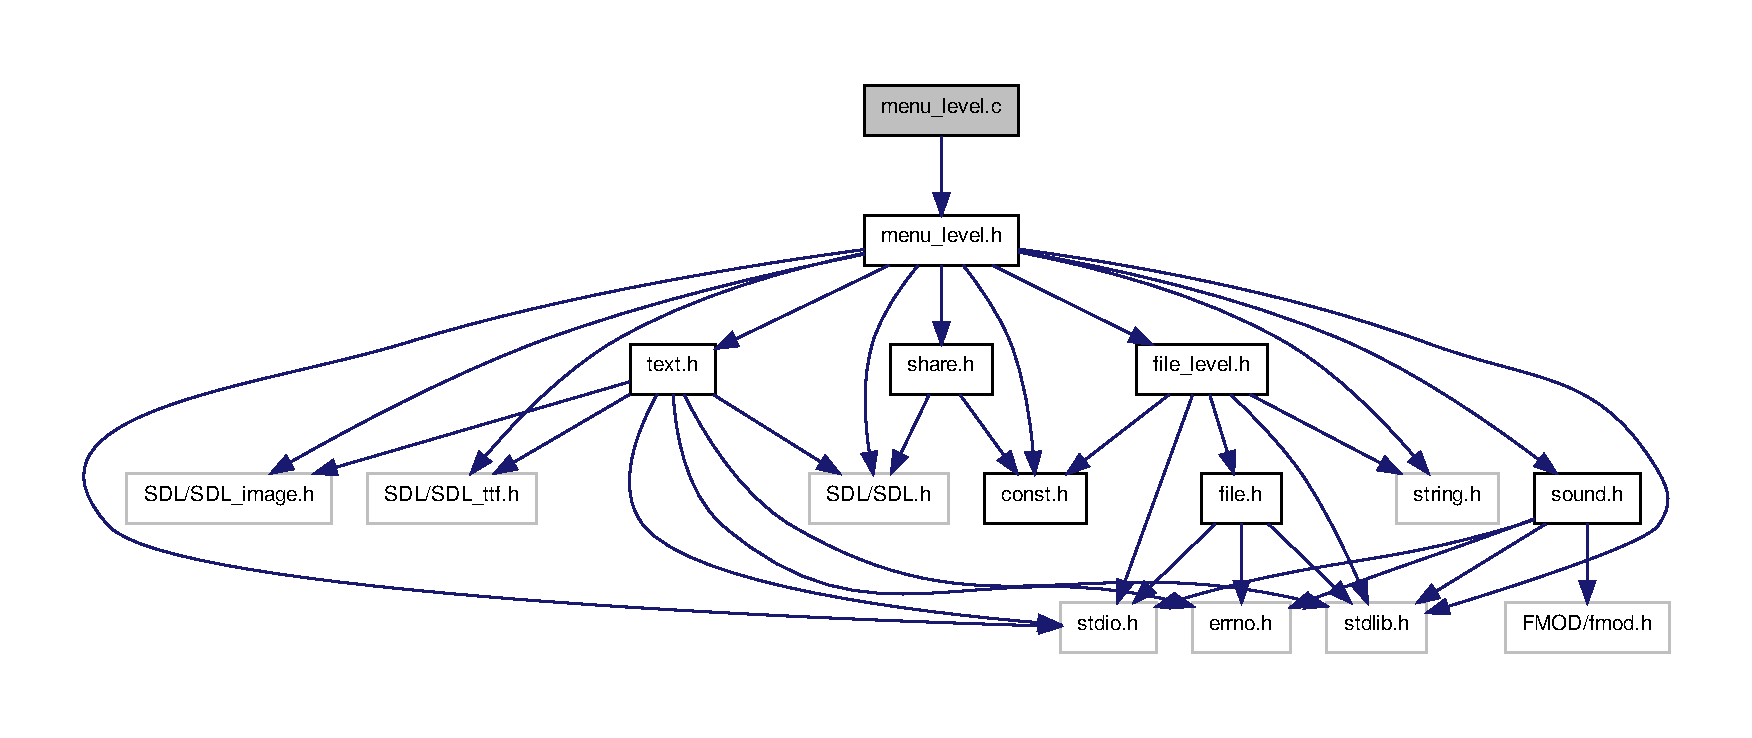
\includegraphics[width=350pt]{menu__level_8c__incl}
\end{center}
\end{figure}
\subsection*{Functions}
\begin{DoxyCompactItemize}
\item 
\hypertarget{menu__level_8c_a794ae7f9d9b9deb8594ec894ef18a2de}{int {\bfseries menu\-Level} (S\-D\-L\-\_\-\-Surface $\ast$screen, char level\-\_\-name\mbox{[}M\-A\-X\-\_\-\-S\-I\-Z\-E\-\_\-\-F\-I\-L\-E\-\_\-\-N\-A\-M\-E\mbox{]}, \hyperlink{struct_sound}{Sound} $\ast$sound\-\_\-sys, char player\-\_\-name\mbox{[}M\-A\-X\-\_\-\-S\-I\-Z\-E\-\_\-\-F\-I\-L\-E\-\_\-\-N\-A\-M\-E\mbox{]}, \hyperlink{struct_player}{Player} $\ast$player, int $\ast$go, int $\ast$nb\-\_\-lvl, \hyperlink{struct_input}{Input} $\ast$in)}\label{menu__level_8c_a794ae7f9d9b9deb8594ec894ef18a2de}

\end{DoxyCompactItemize}


\subsection{Detailed Description}
level choose menu \begin{DoxyAuthor}{Author}
Remi B\-E\-R\-T\-H\-O 
\end{DoxyAuthor}
\begin{DoxyDate}{Date}
15/03/14 
\end{DoxyDate}

\hypertarget{menu__level_8h}{\section{menu\-\_\-level.\-h File Reference}
\label{menu__level_8h}\index{menu\-\_\-level.\-h@{menu\-\_\-level.\-h}}
}


Menu gerant le choix du niveau.  


{\ttfamily \#include $<$stdio.\-h$>$}\\*
{\ttfamily \#include $<$stdlib.\-h$>$}\\*
{\ttfamily \#include $<$string.\-h$>$}\\*
{\ttfamily \#include $<$S\-D\-L/\-S\-D\-L.\-h$>$}\\*
{\ttfamily \#include $<$S\-D\-L/\-S\-D\-L\-\_\-image.\-h$>$}\\*
{\ttfamily \#include $<$S\-D\-L/\-S\-D\-L\-\_\-ttf.\-h$>$}\\*
{\ttfamily \#include \char`\"{}const.\-h\char`\"{}}\\*
{\ttfamily \#include \char`\"{}file\-\_\-level.\-h\char`\"{}}\\*
{\ttfamily \#include \char`\"{}share.\-h\char`\"{}}\\*
{\ttfamily \#include \char`\"{}text.\-h\char`\"{}}\\*
{\ttfamily \#include \char`\"{}sound.\-h\char`\"{}}\\*
Include dependency graph for menu\-\_\-level.\-h\-:
\nopagebreak
\begin{figure}[H]
\begin{center}
\leavevmode
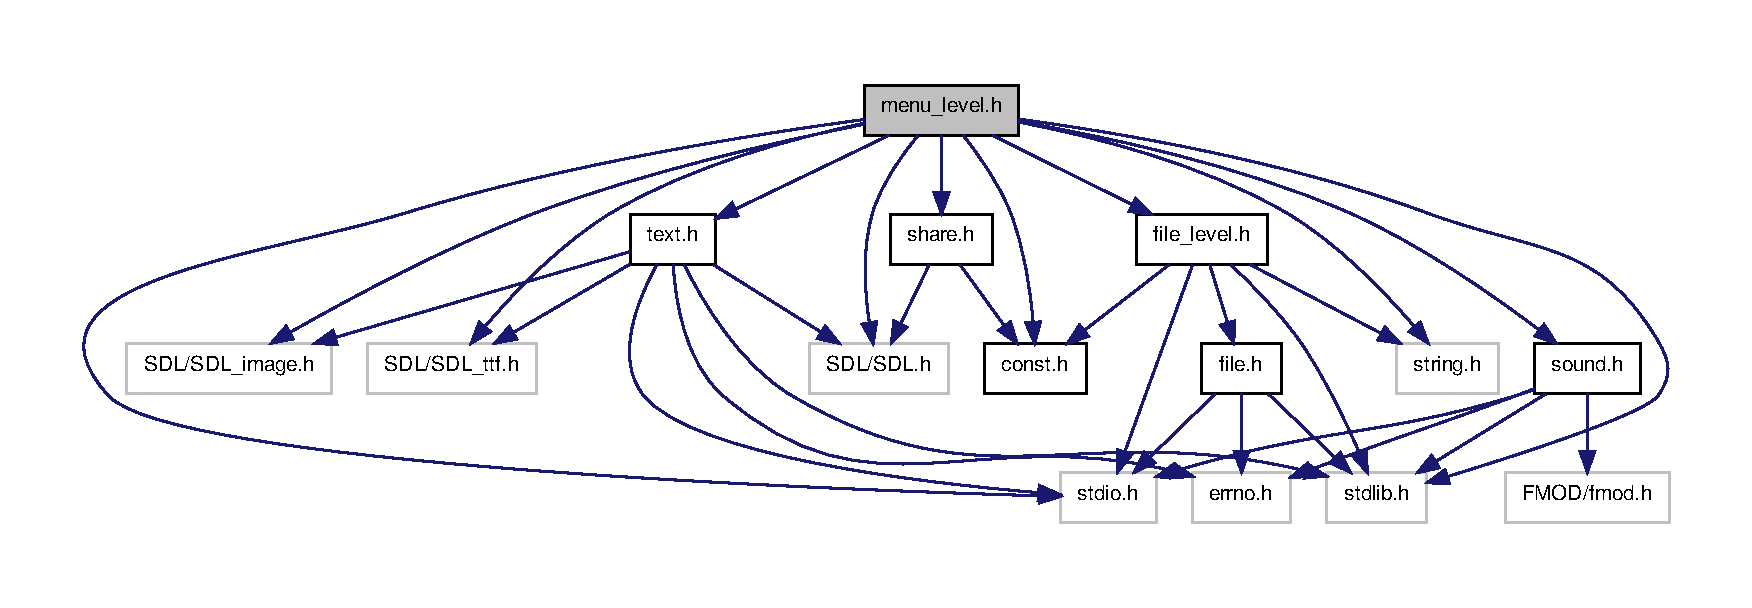
\includegraphics[width=350pt]{menu__level_8h__incl}
\end{center}
\end{figure}
This graph shows which files directly or indirectly include this file\-:
\nopagebreak
\begin{figure}[H]
\begin{center}
\leavevmode
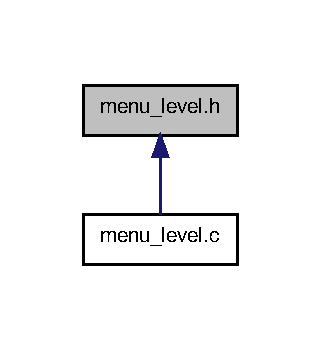
\includegraphics[width=154pt]{menu__level_8h__dep__incl}
\end{center}
\end{figure}
\subsection*{Functions}
\begin{DoxyCompactItemize}
\item 
\hypertarget{menu__level_8h_a2df6ef1e00c1fe9c46d267b8f0f56adf}{int {\bfseries menu\-Level} (S\-D\-L\-\_\-\-Surface $\ast$screen, char level\-\_\-name\mbox{[}T\-A\-I\-L\-L\-E\-\_\-\-M\-A\-X\-\_\-\-N\-O\-M\-\_\-\-F\-I\-C\-H\-I\-E\-R\mbox{]}, \hyperlink{struct_sound}{Sound} $\ast$s)}\label{menu__level_8h_a2df6ef1e00c1fe9c46d267b8f0f56adf}

\end{DoxyCompactItemize}


\subsection{Detailed Description}
Menu gerant le choix du niveau. \begin{DoxyAuthor}{Author}
Remi B\-E\-R\-T\-H\-O 
\end{DoxyAuthor}
\begin{DoxyDate}{Date}
15/03/14 
\end{DoxyDate}
\begin{DoxyVersion}{Version}
1.\-0 
\end{DoxyVersion}

\hypertarget{player_8c}{\subsection{player.\-c File Reference}
\label{player_8c}\index{player.\-c@{player.\-c}}
}


Management of the player system.  


{\ttfamily \#include \char`\"{}player.\-h\char`\"{}}\\*
\subsubsection*{Functions}
\begin{DoxyCompactItemize}
\item 
int \hyperlink{player_8c_a4d30b7faab667544df4847e535dfc6e3}{new\-Player} (S\-D\-L\-\_\-\-Surface $\ast$screen, char player\-\_\-name\mbox{[}\hyperlink{const_8h_a95feb1f1a8c13ebeb7da1e49b2896c24}{M\-A\-X\-\_\-\-S\-I\-Z\-E\-\_\-\-F\-I\-L\-E\-\_\-\-N\-A\-M\-E}\mbox{]}, \hyperlink{struct_sound}{Sound} $\ast$s, int $\ast$go)
\item 
void \hyperlink{player_8c_a8330f47dea4a7c01a97ecef3607c3448}{load\-Player} (char file\-Save\mbox{[}\hyperlink{const_8h_a95feb1f1a8c13ebeb7da1e49b2896c24}{M\-A\-X\-\_\-\-S\-I\-Z\-E\-\_\-\-F\-I\-L\-E\-\_\-\-N\-A\-M\-E}\mbox{]}, char player\-\_\-name\mbox{[}\hyperlink{const_8h_a95feb1f1a8c13ebeb7da1e49b2896c24}{M\-A\-X\-\_\-\-S\-I\-Z\-E\-\_\-\-F\-I\-L\-E\-\_\-\-N\-A\-M\-E}\mbox{]}, \hyperlink{struct_player}{Player} $\ast$player)
\item 
int \hyperlink{player_8c_ac02b9148199bc3334b6c7149789c946c}{save\-Player} (char file\-Save\mbox{[}\hyperlink{const_8h_a95feb1f1a8c13ebeb7da1e49b2896c24}{M\-A\-X\-\_\-\-S\-I\-Z\-E\-\_\-\-F\-I\-L\-E\-\_\-\-N\-A\-M\-E}\mbox{]}, char player\-\_\-name\mbox{[}\hyperlink{const_8h_a95feb1f1a8c13ebeb7da1e49b2896c24}{M\-A\-X\-\_\-\-S\-I\-Z\-E\-\_\-\-F\-I\-L\-E\-\_\-\-N\-A\-M\-E}\mbox{]}, \hyperlink{struct_player}{Player} $\ast$player)
\item 
void \hyperlink{player_8c_a5bb0205907acbfde9bc8a6935e9da97e}{save} (S\-D\-L\-\_\-\-Surface $\ast$screen, char file\-Save\mbox{[}\hyperlink{const_8h_a95feb1f1a8c13ebeb7da1e49b2896c24}{M\-A\-X\-\_\-\-S\-I\-Z\-E\-\_\-\-F\-I\-L\-E\-\_\-\-N\-A\-M\-E}\mbox{]}, char player\-\_\-name\mbox{[}\hyperlink{const_8h_a95feb1f1a8c13ebeb7da1e49b2896c24}{M\-A\-X\-\_\-\-S\-I\-Z\-E\-\_\-\-F\-I\-L\-E\-\_\-\-N\-A\-M\-E}\mbox{]}, \hyperlink{struct_player}{Player} $\ast$player, int $\ast$go)
\item 
void \hyperlink{player_8c_a759d67ed182fea0f5ec9d9722c188336}{delete\-Player} (S\-D\-L\-\_\-\-Surface $\ast$screen, char file\-Save\mbox{[}\hyperlink{const_8h_a95feb1f1a8c13ebeb7da1e49b2896c24}{M\-A\-X\-\_\-\-S\-I\-Z\-E\-\_\-\-F\-I\-L\-E\-\_\-\-N\-A\-M\-E}\mbox{]}, char player\-\_\-name\mbox{[}\hyperlink{const_8h_a95feb1f1a8c13ebeb7da1e49b2896c24}{M\-A\-X\-\_\-\-S\-I\-Z\-E\-\_\-\-F\-I\-L\-E\-\_\-\-N\-A\-M\-E}\mbox{]})
\end{DoxyCompactItemize}


\subsubsection{Detailed Description}
Management of the player system. \begin{DoxyAuthor}{Author}
Glenn H\-E\-R\-R\-O\-U 
\end{DoxyAuthor}
\begin{DoxyDate}{Date}
06/05/14 
\end{DoxyDate}
\begin{DoxyVersion}{Version}
1.\-0 
\end{DoxyVersion}


\subsubsection{Function Documentation}
\hypertarget{player_8c_a759d67ed182fea0f5ec9d9722c188336}{\index{player.\-c@{player.\-c}!delete\-Player@{delete\-Player}}
\index{delete\-Player@{delete\-Player}!player.c@{player.\-c}}
\paragraph[{delete\-Player}]{\setlength{\rightskip}{0pt plus 5cm}void delete\-Player (
\begin{DoxyParamCaption}
\item[{S\-D\-L\-\_\-\-Surface $\ast$}]{screen, }
\item[{char}]{file\-Save\mbox{[}\-M\-A\-X\-\_\-\-S\-I\-Z\-E\-\_\-\-F\-I\-L\-E\-\_\-\-N\-A\-M\-E\mbox{]}, }
\item[{char}]{player\-\_\-name\mbox{[}\-M\-A\-X\-\_\-\-S\-I\-Z\-E\-\_\-\-F\-I\-L\-E\-\_\-\-N\-A\-M\-E\mbox{]}}
\end{DoxyParamCaption}
)}}\label{player_8c_a759d67ed182fea0f5ec9d9722c188336}
Delete the current player in the player list. 
\begin{DoxyParams}[1]{Parameters}
\mbox{\tt in,out}  & {\em screen} & The screen of the game \\
\hline
\mbox{\tt in,out}  & {\em file\-Save} & The path to the binary file containing the progression of each player \\
\hline
\mbox{\tt in}  & {\em player\-\_\-name} & The name of the current player \\
\hline
\end{DoxyParams}


Here is the call graph for this function\-:
\nopagebreak
\begin{figure}[H]
\begin{center}
\leavevmode
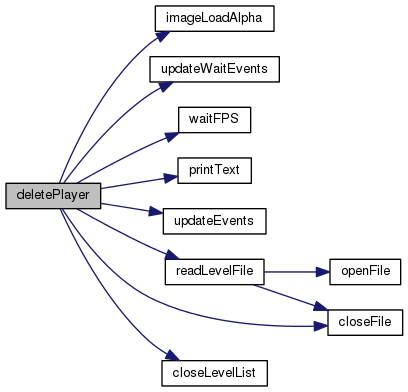
\includegraphics[width=350pt]{player_8c_a759d67ed182fea0f5ec9d9722c188336_cgraph}
\end{center}
\end{figure}


\hypertarget{player_8c_a8330f47dea4a7c01a97ecef3607c3448}{\index{player.\-c@{player.\-c}!load\-Player@{load\-Player}}
\index{load\-Player@{load\-Player}!player.c@{player.\-c}}
\paragraph[{load\-Player}]{\setlength{\rightskip}{0pt plus 5cm}void load\-Player (
\begin{DoxyParamCaption}
\item[{char}]{file\-Save\mbox{[}\-M\-A\-X\-\_\-\-S\-I\-Z\-E\-\_\-\-F\-I\-L\-E\-\_\-\-N\-A\-M\-E\mbox{]}, }
\item[{char}]{player\-\_\-name\mbox{[}\-M\-A\-X\-\_\-\-S\-I\-Z\-E\-\_\-\-F\-I\-L\-E\-\_\-\-N\-A\-M\-E\mbox{]}, }
\item[{{\bf Player} $\ast$}]{player}
\end{DoxyParamCaption}
)}}\label{player_8c_a8330f47dea4a7c01a97ecef3607c3448}
Load the progression of the given player from the binary file named file\-Save 
\begin{DoxyParams}[1]{Parameters}
\mbox{\tt in}  & {\em file\-Save} & The path to the binary file containing the progression of each player \\
\hline
\mbox{\tt in}  & {\em player\-\_\-name} & The name of the current player \\
\hline
\mbox{\tt out}  & {\em player} & The player structure where the progression will be loaded \\
\hline
\end{DoxyParams}
\hypertarget{player_8c_a4d30b7faab667544df4847e535dfc6e3}{\index{player.\-c@{player.\-c}!new\-Player@{new\-Player}}
\index{new\-Player@{new\-Player}!player.c@{player.\-c}}
\paragraph[{new\-Player}]{\setlength{\rightskip}{0pt plus 5cm}int new\-Player (
\begin{DoxyParamCaption}
\item[{S\-D\-L\-\_\-\-Surface $\ast$}]{screen, }
\item[{char}]{player\-\_\-name\mbox{[}\-M\-A\-X\-\_\-\-S\-I\-Z\-E\-\_\-\-F\-I\-L\-E\-\_\-\-N\-A\-M\-E\mbox{]}, }
\item[{{\bf Sound} $\ast$}]{s, }
\item[{int $\ast$}]{go}
\end{DoxyParamCaption}
)}}\label{player_8c_a4d30b7faab667544df4847e535dfc6e3}
Display the interface to create a new player 
\begin{DoxyParams}[1]{Parameters}
\mbox{\tt in,out}  & {\em screen} & The screen of the game \\
\hline
\mbox{\tt out}  & {\em player\-\_\-name} & The name of the new player \\
\hline
\mbox{\tt out}  & {\em s} & the sound system \\
\hline
\mbox{\tt out}  & {\em go} & the main loop validation \\
\hline
\end{DoxyParams}
\begin{DoxyReturn}{Returns}
1 if a new player has been created, 0 otherwise 
\end{DoxyReturn}


Here is the call graph for this function\-:
\nopagebreak
\begin{figure}[H]
\begin{center}
\leavevmode
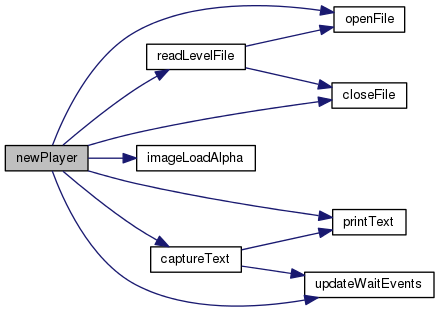
\includegraphics[width=350pt]{player_8c_a4d30b7faab667544df4847e535dfc6e3_cgraph}
\end{center}
\end{figure}


\hypertarget{player_8c_a5bb0205907acbfde9bc8a6935e9da97e}{\index{player.\-c@{player.\-c}!save@{save}}
\index{save@{save}!player.c@{player.\-c}}
\paragraph[{save}]{\setlength{\rightskip}{0pt plus 5cm}void save (
\begin{DoxyParamCaption}
\item[{S\-D\-L\-\_\-\-Surface $\ast$}]{screen, }
\item[{char}]{file\-Save\mbox{[}\-M\-A\-X\-\_\-\-S\-I\-Z\-E\-\_\-\-F\-I\-L\-E\-\_\-\-N\-A\-M\-E\mbox{]}, }
\item[{char}]{player\-\_\-name\mbox{[}\-M\-A\-X\-\_\-\-S\-I\-Z\-E\-\_\-\-F\-I\-L\-E\-\_\-\-N\-A\-M\-E\mbox{]}, }
\item[{{\bf Player} $\ast$}]{player, }
\item[{int $\ast$}]{go}
\end{DoxyParamCaption}
)}}\label{player_8c_a5bb0205907acbfde9bc8a6935e9da97e}
Display the interface to save the player progression 
\begin{DoxyParams}[1]{Parameters}
\mbox{\tt in,out}  & {\em screen} & The screen of the game \\
\hline
\mbox{\tt in}  & {\em file\-Save} & The path to the binary file containing the progression of each player \\
\hline
\mbox{\tt in}  & {\em player\-\_\-name} & The name of the current player \\
\hline
\mbox{\tt out}  & {\em player} & The player structure where the progression is stored \\
\hline
\mbox{\tt out}  & {\em go} & The main loop validation \\
\hline
\end{DoxyParams}


Here is the call graph for this function\-:
\nopagebreak
\begin{figure}[H]
\begin{center}
\leavevmode
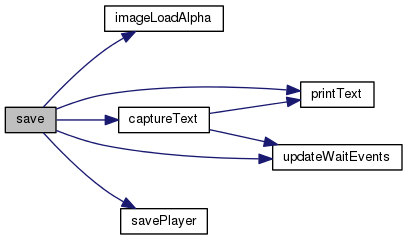
\includegraphics[width=350pt]{player_8c_a5bb0205907acbfde9bc8a6935e9da97e_cgraph}
\end{center}
\end{figure}


\hypertarget{player_8c_ac02b9148199bc3334b6c7149789c946c}{\index{player.\-c@{player.\-c}!save\-Player@{save\-Player}}
\index{save\-Player@{save\-Player}!player.c@{player.\-c}}
\paragraph[{save\-Player}]{\setlength{\rightskip}{0pt plus 5cm}int save\-Player (
\begin{DoxyParamCaption}
\item[{char}]{file\-Save\mbox{[}\-M\-A\-X\-\_\-\-S\-I\-Z\-E\-\_\-\-F\-I\-L\-E\-\_\-\-N\-A\-M\-E\mbox{]}, }
\item[{char}]{player\-\_\-name\mbox{[}\-M\-A\-X\-\_\-\-S\-I\-Z\-E\-\_\-\-F\-I\-L\-E\-\_\-\-N\-A\-M\-E\mbox{]}, }
\item[{{\bf Player} $\ast$}]{player}
\end{DoxyParamCaption}
)}}\label{player_8c_ac02b9148199bc3334b6c7149789c946c}
Save the progression of the given player in the binary file named file\-Save 
\begin{DoxyParams}[1]{Parameters}
\mbox{\tt in}  & {\em file\-Save} & The path to the binary file containing the progression of each player \\
\hline
\mbox{\tt in}  & {\em player\-\_\-name} & The name of the current player \\
\hline
\mbox{\tt out}  & {\em player} & The player structure where the progression is stored \\
\hline
\end{DoxyParams}

\hypertarget{player_8h}{\subsection{player.\-h File Reference}
\label{player_8h}\index{player.\-h@{player.\-h}}
}


\hyperlink{player_8c}{player.\-c} header  


{\ttfamily \#include $<$stdio.\-h$>$}\\*
{\ttfamily \#include $<$stdlib.\-h$>$}\\*
{\ttfamily \#include $<$string.\-h$>$}\\*
{\ttfamily \#include $<$S\-D\-L/\-S\-D\-L.\-h$>$}\\*
{\ttfamily \#include $<$S\-D\-L/\-S\-D\-L\-\_\-image.\-h$>$}\\*
{\ttfamily \#include $<$S\-D\-L/\-S\-D\-L\-\_\-ttf.\-h$>$}\\*
{\ttfamily \#include \char`\"{}const.\-h\char`\"{}}\\*
{\ttfamily \#include \char`\"{}structures.\-h\char`\"{}}\\*
{\ttfamily \#include \char`\"{}file\-\_\-level.\-h\char`\"{}}\\*
{\ttfamily \#include \char`\"{}share.\-h\char`\"{}}\\*
{\ttfamily \#include \char`\"{}text.\-h\char`\"{}}\\*
{\ttfamily \#include \char`\"{}sound.\-h\char`\"{}}\\*
{\ttfamily \#include \char`\"{}image.\-h\char`\"{}}\\*
{\ttfamily \#include \char`\"{}input.\-h\char`\"{}}\\*
\subsubsection*{Functions}
\begin{DoxyCompactItemize}
\item 
int \hyperlink{player_8h_a4d30b7faab667544df4847e535dfc6e3}{new\-Player} (S\-D\-L\-\_\-\-Surface $\ast$screen, char player\-\_\-name\mbox{[}\hyperlink{const_8h_a95feb1f1a8c13ebeb7da1e49b2896c24}{M\-A\-X\-\_\-\-S\-I\-Z\-E\-\_\-\-F\-I\-L\-E\-\_\-\-N\-A\-M\-E}\mbox{]}, \hyperlink{struct_sound}{Sound} $\ast$s, int $\ast$go)
\item 
void \hyperlink{player_8h_a8330f47dea4a7c01a97ecef3607c3448}{load\-Player} (char file\-Save\mbox{[}\hyperlink{const_8h_a95feb1f1a8c13ebeb7da1e49b2896c24}{M\-A\-X\-\_\-\-S\-I\-Z\-E\-\_\-\-F\-I\-L\-E\-\_\-\-N\-A\-M\-E}\mbox{]}, char player\-\_\-name\mbox{[}\hyperlink{const_8h_a95feb1f1a8c13ebeb7da1e49b2896c24}{M\-A\-X\-\_\-\-S\-I\-Z\-E\-\_\-\-F\-I\-L\-E\-\_\-\-N\-A\-M\-E}\mbox{]}, \hyperlink{struct_player}{Player} $\ast$player)
\item 
int \hyperlink{player_8h_ac02b9148199bc3334b6c7149789c946c}{save\-Player} (char file\-Save\mbox{[}\hyperlink{const_8h_a95feb1f1a8c13ebeb7da1e49b2896c24}{M\-A\-X\-\_\-\-S\-I\-Z\-E\-\_\-\-F\-I\-L\-E\-\_\-\-N\-A\-M\-E}\mbox{]}, char player\-\_\-name\mbox{[}\hyperlink{const_8h_a95feb1f1a8c13ebeb7da1e49b2896c24}{M\-A\-X\-\_\-\-S\-I\-Z\-E\-\_\-\-F\-I\-L\-E\-\_\-\-N\-A\-M\-E}\mbox{]}, \hyperlink{struct_player}{Player} $\ast$player)
\item 
void \hyperlink{player_8h_a5bb0205907acbfde9bc8a6935e9da97e}{save} (S\-D\-L\-\_\-\-Surface $\ast$screen, char file\-Save\mbox{[}\hyperlink{const_8h_a95feb1f1a8c13ebeb7da1e49b2896c24}{M\-A\-X\-\_\-\-S\-I\-Z\-E\-\_\-\-F\-I\-L\-E\-\_\-\-N\-A\-M\-E}\mbox{]}, char player\-\_\-name\mbox{[}\hyperlink{const_8h_a95feb1f1a8c13ebeb7da1e49b2896c24}{M\-A\-X\-\_\-\-S\-I\-Z\-E\-\_\-\-F\-I\-L\-E\-\_\-\-N\-A\-M\-E}\mbox{]}, \hyperlink{struct_player}{Player} $\ast$player, int $\ast$go)
\item 
void \hyperlink{player_8h_a759d67ed182fea0f5ec9d9722c188336}{delete\-Player} (S\-D\-L\-\_\-\-Surface $\ast$screen, char file\-Save\mbox{[}\hyperlink{const_8h_a95feb1f1a8c13ebeb7da1e49b2896c24}{M\-A\-X\-\_\-\-S\-I\-Z\-E\-\_\-\-F\-I\-L\-E\-\_\-\-N\-A\-M\-E}\mbox{]}, char player\-\_\-name\mbox{[}\hyperlink{const_8h_a95feb1f1a8c13ebeb7da1e49b2896c24}{M\-A\-X\-\_\-\-S\-I\-Z\-E\-\_\-\-F\-I\-L\-E\-\_\-\-N\-A\-M\-E}\mbox{]})
\end{DoxyCompactItemize}


\subsubsection{Detailed Description}
\hyperlink{player_8c}{player.\-c} header \begin{DoxyAuthor}{Author}
Glenn H\-E\-R\-R\-O\-U 
\end{DoxyAuthor}
\begin{DoxyDate}{Date}
06/05/14 
\end{DoxyDate}
\begin{DoxyVersion}{Version}
1.\-0 
\end{DoxyVersion}


\subsubsection{Function Documentation}
\hypertarget{player_8h_a759d67ed182fea0f5ec9d9722c188336}{\index{player.\-h@{player.\-h}!delete\-Player@{delete\-Player}}
\index{delete\-Player@{delete\-Player}!player.h@{player.\-h}}
\paragraph[{delete\-Player}]{\setlength{\rightskip}{0pt plus 5cm}void delete\-Player (
\begin{DoxyParamCaption}
\item[{S\-D\-L\-\_\-\-Surface $\ast$}]{screen, }
\item[{char}]{file\-Save\mbox{[}\-M\-A\-X\-\_\-\-S\-I\-Z\-E\-\_\-\-F\-I\-L\-E\-\_\-\-N\-A\-M\-E\mbox{]}, }
\item[{char}]{player\-\_\-name\mbox{[}\-M\-A\-X\-\_\-\-S\-I\-Z\-E\-\_\-\-F\-I\-L\-E\-\_\-\-N\-A\-M\-E\mbox{]}}
\end{DoxyParamCaption}
)}}\label{player_8h_a759d67ed182fea0f5ec9d9722c188336}
Delete the current player in the player list. 
\begin{DoxyParams}[1]{Parameters}
\mbox{\tt in,out}  & {\em screen} & The screen of the game \\
\hline
\mbox{\tt in,out}  & {\em file\-Save} & The path to the binary file containing the progression of each player \\
\hline
\mbox{\tt in}  & {\em player\-\_\-name} & The name of the current player \\
\hline
\end{DoxyParams}


Here is the call graph for this function\-:
\nopagebreak
\begin{figure}[H]
\begin{center}
\leavevmode
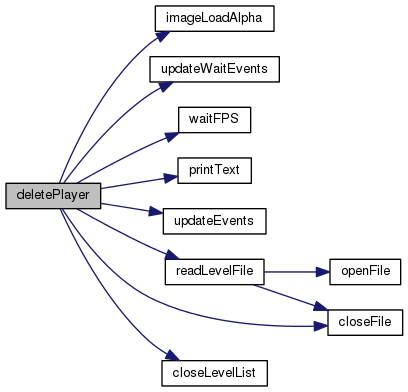
\includegraphics[width=350pt]{player_8h_a759d67ed182fea0f5ec9d9722c188336_cgraph}
\end{center}
\end{figure}


\hypertarget{player_8h_a8330f47dea4a7c01a97ecef3607c3448}{\index{player.\-h@{player.\-h}!load\-Player@{load\-Player}}
\index{load\-Player@{load\-Player}!player.h@{player.\-h}}
\paragraph[{load\-Player}]{\setlength{\rightskip}{0pt plus 5cm}void load\-Player (
\begin{DoxyParamCaption}
\item[{char}]{file\-Save\mbox{[}\-M\-A\-X\-\_\-\-S\-I\-Z\-E\-\_\-\-F\-I\-L\-E\-\_\-\-N\-A\-M\-E\mbox{]}, }
\item[{char}]{player\-\_\-name\mbox{[}\-M\-A\-X\-\_\-\-S\-I\-Z\-E\-\_\-\-F\-I\-L\-E\-\_\-\-N\-A\-M\-E\mbox{]}, }
\item[{{\bf Player} $\ast$}]{player}
\end{DoxyParamCaption}
)}}\label{player_8h_a8330f47dea4a7c01a97ecef3607c3448}
Load the progression of the given player from the binary file named file\-Save 
\begin{DoxyParams}[1]{Parameters}
\mbox{\tt in}  & {\em file\-Save} & The path to the binary file containing the progression of each player \\
\hline
\mbox{\tt in}  & {\em player\-\_\-name} & The name of the current player \\
\hline
\mbox{\tt out}  & {\em player} & The player structure where the progression will be loaded \\
\hline
\end{DoxyParams}
\hypertarget{player_8h_a4d30b7faab667544df4847e535dfc6e3}{\index{player.\-h@{player.\-h}!new\-Player@{new\-Player}}
\index{new\-Player@{new\-Player}!player.h@{player.\-h}}
\paragraph[{new\-Player}]{\setlength{\rightskip}{0pt plus 5cm}int new\-Player (
\begin{DoxyParamCaption}
\item[{S\-D\-L\-\_\-\-Surface $\ast$}]{screen, }
\item[{char}]{player\-\_\-name\mbox{[}\-M\-A\-X\-\_\-\-S\-I\-Z\-E\-\_\-\-F\-I\-L\-E\-\_\-\-N\-A\-M\-E\mbox{]}, }
\item[{{\bf Sound} $\ast$}]{s, }
\item[{int $\ast$}]{go}
\end{DoxyParamCaption}
)}}\label{player_8h_a4d30b7faab667544df4847e535dfc6e3}
Display the interface to create a new player 
\begin{DoxyParams}[1]{Parameters}
\mbox{\tt in,out}  & {\em screen} & The screen of the game \\
\hline
\mbox{\tt out}  & {\em player\-\_\-name} & The name of the new player \\
\hline
\mbox{\tt out}  & {\em s} & the sound system \\
\hline
\mbox{\tt out}  & {\em go} & the main loop validation \\
\hline
\end{DoxyParams}
\begin{DoxyReturn}{Returns}
1 if a new player has been created, 0 otherwise 
\end{DoxyReturn}


Here is the call graph for this function\-:
\nopagebreak
\begin{figure}[H]
\begin{center}
\leavevmode
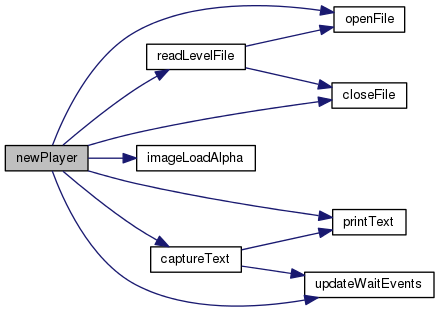
\includegraphics[width=350pt]{player_8h_a4d30b7faab667544df4847e535dfc6e3_cgraph}
\end{center}
\end{figure}


\hypertarget{player_8h_a5bb0205907acbfde9bc8a6935e9da97e}{\index{player.\-h@{player.\-h}!save@{save}}
\index{save@{save}!player.h@{player.\-h}}
\paragraph[{save}]{\setlength{\rightskip}{0pt plus 5cm}void save (
\begin{DoxyParamCaption}
\item[{S\-D\-L\-\_\-\-Surface $\ast$}]{screen, }
\item[{char}]{file\-Save\mbox{[}\-M\-A\-X\-\_\-\-S\-I\-Z\-E\-\_\-\-F\-I\-L\-E\-\_\-\-N\-A\-M\-E\mbox{]}, }
\item[{char}]{player\-\_\-name\mbox{[}\-M\-A\-X\-\_\-\-S\-I\-Z\-E\-\_\-\-F\-I\-L\-E\-\_\-\-N\-A\-M\-E\mbox{]}, }
\item[{{\bf Player} $\ast$}]{player, }
\item[{int $\ast$}]{go}
\end{DoxyParamCaption}
)}}\label{player_8h_a5bb0205907acbfde9bc8a6935e9da97e}
Display the interface to save the player progression 
\begin{DoxyParams}[1]{Parameters}
\mbox{\tt in,out}  & {\em screen} & The screen of the game \\
\hline
\mbox{\tt in}  & {\em file\-Save} & The path to the binary file containing the progression of each player \\
\hline
\mbox{\tt in}  & {\em player\-\_\-name} & The name of the current player \\
\hline
\mbox{\tt out}  & {\em player} & The player structure where the progression is stored \\
\hline
\mbox{\tt out}  & {\em go} & The main loop validation \\
\hline
\end{DoxyParams}


Here is the call graph for this function\-:
\nopagebreak
\begin{figure}[H]
\begin{center}
\leavevmode
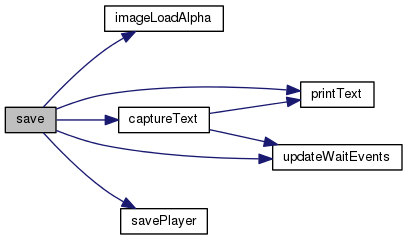
\includegraphics[width=350pt]{player_8h_a5bb0205907acbfde9bc8a6935e9da97e_cgraph}
\end{center}
\end{figure}


\hypertarget{player_8h_ac02b9148199bc3334b6c7149789c946c}{\index{player.\-h@{player.\-h}!save\-Player@{save\-Player}}
\index{save\-Player@{save\-Player}!player.h@{player.\-h}}
\paragraph[{save\-Player}]{\setlength{\rightskip}{0pt plus 5cm}int save\-Player (
\begin{DoxyParamCaption}
\item[{char}]{file\-Save\mbox{[}\-M\-A\-X\-\_\-\-S\-I\-Z\-E\-\_\-\-F\-I\-L\-E\-\_\-\-N\-A\-M\-E\mbox{]}, }
\item[{char}]{player\-\_\-name\mbox{[}\-M\-A\-X\-\_\-\-S\-I\-Z\-E\-\_\-\-F\-I\-L\-E\-\_\-\-N\-A\-M\-E\mbox{]}, }
\item[{{\bf Player} $\ast$}]{player}
\end{DoxyParamCaption}
)}}\label{player_8h_ac02b9148199bc3334b6c7149789c946c}
Save the progression of the given player in the binary file named file\-Save 
\begin{DoxyParams}[1]{Parameters}
\mbox{\tt in}  & {\em file\-Save} & The path to the binary file containing the progression of each player \\
\hline
\mbox{\tt in}  & {\em player\-\_\-name} & The name of the current player \\
\hline
\mbox{\tt out}  & {\em player} & The player structure where the progression is stored \\
\hline
\end{DoxyParams}

\hypertarget{sound_8c}{\section{sound.\-c File Reference}
\label{sound_8c}\index{sound.\-c@{sound.\-c}}
}


contient les fonction pour jouer du son  


{\ttfamily \#include \char`\"{}sound.\-h\char`\"{}}\\*
Include dependency graph for sound.\-c\-:\nopagebreak
\begin{figure}[H]
\begin{center}
\leavevmode
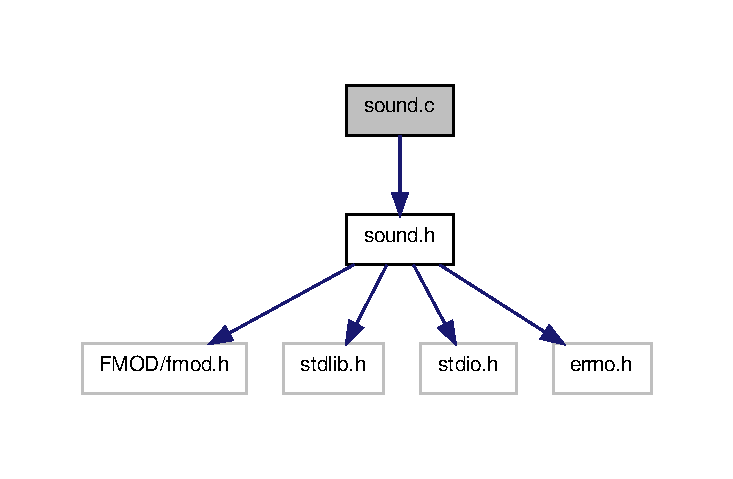
\includegraphics[width=350pt]{sound_8c__incl}
\end{center}
\end{figure}
\subsection*{Functions}
\begin{DoxyCompactItemize}
\item 
\hyperlink{struct_sound}{Sound} $\ast$ \hyperlink{sound_8c_a3b1e12665aed7169d8efdb2cc611184e}{create\-Sound} (void)
\item 
void \hyperlink{sound_8c_a3af6fda5716d5f42846d0ccc01d5e2ca}{play\-Music} (\hyperlink{struct_sound}{Sound} $\ast$s, char $\ast$file)
\item 
void \hyperlink{sound_8c_a5378cbd0e1d0bfeaa823df1a8ea215f3}{play\-Music\-Once} (\hyperlink{struct_sound}{Sound} $\ast$s, char $\ast$file)
\item 
void \hyperlink{sound_8c_acc13f1ac1e0bac5afe39405869772a08}{free\-Sound} (\hyperlink{struct_sound}{Sound} $\ast$s)
\item 
void \hyperlink{sound_8c_ac3737f55b80ac35471d115d0304e8bc3}{stop\-Sound} (\hyperlink{struct_sound}{Sound} $\ast$s)
\item 
void \hyperlink{sound_8c_a63831c086cacea9358f5c86bebbfb288}{sound\-Volume} (\hyperlink{struct_sound}{Sound} $\ast$s, float volume)
\end{DoxyCompactItemize}


\subsection{Detailed Description}
contient les fonction pour jouer du son \begin{DoxyAuthor}{Author}
Xavier C\-O\-P\-O\-N\-E\-T 
\end{DoxyAuthor}
\begin{DoxyDate}{Date}
2014-\/02-\/27 
\end{DoxyDate}


\subsection{Function Documentation}
\hypertarget{sound_8c_a3b1e12665aed7169d8efdb2cc611184e}{\index{sound.\-c@{sound.\-c}!create\-Sound@{create\-Sound}}
\index{create\-Sound@{create\-Sound}!sound.c@{sound.\-c}}
\subsubsection[{create\-Sound}]{\setlength{\rightskip}{0pt plus 5cm}sound $\ast$ create\-Sound (
\begin{DoxyParamCaption}
\item[{void}]{}
\end{DoxyParamCaption}
)}}\label{sound_8c_a3b1e12665aed7169d8efdb2cc611184e}
créer une structure son \begin{DoxyReturn}{Returns}
la structure son 
\end{DoxyReturn}
\hypertarget{sound_8c_acc13f1ac1e0bac5afe39405869772a08}{\index{sound.\-c@{sound.\-c}!free\-Sound@{free\-Sound}}
\index{free\-Sound@{free\-Sound}!sound.c@{sound.\-c}}
\subsubsection[{free\-Sound}]{\setlength{\rightskip}{0pt plus 5cm}void free\-Sound (
\begin{DoxyParamCaption}
\item[{{\bf Sound} $\ast$}]{s}
\end{DoxyParamCaption}
)}}\label{sound_8c_acc13f1ac1e0bac5afe39405869772a08}
release the sound 
\begin{DoxyParams}[1]{Parameters}
\mbox{\tt out}  & {\em s} & the sound \\
\hline
\end{DoxyParams}
\hypertarget{sound_8c_a3af6fda5716d5f42846d0ccc01d5e2ca}{\index{sound.\-c@{sound.\-c}!play\-Music@{play\-Music}}
\index{play\-Music@{play\-Music}!sound.c@{sound.\-c}}
\subsubsection[{play\-Music}]{\setlength{\rightskip}{0pt plus 5cm}void play\-Music (
\begin{DoxyParamCaption}
\item[{{\bf Sound} $\ast$}]{s, }
\item[{char $\ast$}]{file}
\end{DoxyParamCaption}
)}}\label{sound_8c_a3af6fda5716d5f42846d0ccc01d5e2ca}
lit un fichier long (musique) 
\begin{DoxyParams}[1]{Parameters}
\mbox{\tt in,out}  & {\em s} & la structure son que l'on manipule \\
\hline
\mbox{\tt in}  & {\em file} & Le fichier son à lire \\
\hline
\end{DoxyParams}
\hypertarget{sound_8c_a5378cbd0e1d0bfeaa823df1a8ea215f3}{\index{sound.\-c@{sound.\-c}!play\-Music\-Once@{play\-Music\-Once}}
\index{play\-Music\-Once@{play\-Music\-Once}!sound.c@{sound.\-c}}
\subsubsection[{play\-Music\-Once}]{\setlength{\rightskip}{0pt plus 5cm}void play\-Music\-Once (
\begin{DoxyParamCaption}
\item[{{\bf Sound} $\ast$}]{s, }
\item[{char $\ast$}]{file}
\end{DoxyParamCaption}
)}}\label{sound_8c_a5378cbd0e1d0bfeaa823df1a8ea215f3}
lit un fichier long une fois 
\begin{DoxyParams}[1]{Parameters}
\mbox{\tt in,out}  & {\em s} & la structure son que l'on manipule \\
\hline
\mbox{\tt in}  & {\em file} & Le fichier son à lire \\
\hline
\end{DoxyParams}
\hypertarget{sound_8c_a63831c086cacea9358f5c86bebbfb288}{\index{sound.\-c@{sound.\-c}!sound\-Volume@{sound\-Volume}}
\index{sound\-Volume@{sound\-Volume}!sound.c@{sound.\-c}}
\subsubsection[{sound\-Volume}]{\setlength{\rightskip}{0pt plus 5cm}void sound\-Volume (
\begin{DoxyParamCaption}
\item[{{\bf Sound} $\ast$}]{s, }
\item[{float}]{volume}
\end{DoxyParamCaption}
)}}\label{sound_8c_a63831c086cacea9358f5c86bebbfb288}
set the sound volume 
\begin{DoxyParams}[1]{Parameters}
\mbox{\tt out}  & {\em s} & the sound \\
\hline
\mbox{\tt in}  & {\em volume} & the sound volume \-: \mbox{[}0.\-0 \-: no sound ; 1.\-0 (default) max power\mbox{]} \\
\hline
\end{DoxyParams}
\hypertarget{sound_8c_ac3737f55b80ac35471d115d0304e8bc3}{\index{sound.\-c@{sound.\-c}!stop\-Sound@{stop\-Sound}}
\index{stop\-Sound@{stop\-Sound}!sound.c@{sound.\-c}}
\subsubsection[{stop\-Sound}]{\setlength{\rightskip}{0pt plus 5cm}void stop\-Sound (
\begin{DoxyParamCaption}
\item[{{\bf Sound} $\ast$}]{s}
\end{DoxyParamCaption}
)}}\label{sound_8c_ac3737f55b80ac35471d115d0304e8bc3}
stop the sound 
\begin{DoxyParams}[1]{Parameters}
\mbox{\tt out}  & {\em the} & sound to stop \\
\hline
\end{DoxyParams}

\hypertarget{sound_8h}{\section{sound.\-h File Reference}
\label{sound_8h}\index{sound.\-h@{sound.\-h}}
}


header de \hyperlink{sound_8c}{sound.\-c}  


{\ttfamily \#include $<$F\-M\-O\-D/fmod.\-h$>$}\\*
{\ttfamily \#include $<$stdlib.\-h$>$}\\*
{\ttfamily \#include $<$stdio.\-h$>$}\\*
{\ttfamily \#include $<$errno.\-h$>$}\\*
Include dependency graph for sound.\-h\-:\nopagebreak
\begin{figure}[H]
\begin{center}
\leavevmode
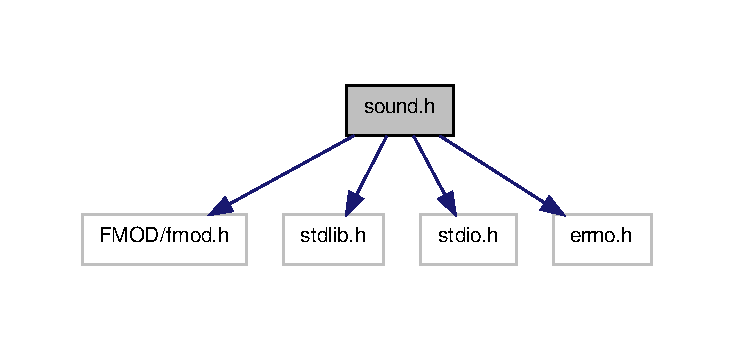
\includegraphics[width=350pt]{sound_8h__incl}
\end{center}
\end{figure}
This graph shows which files directly or indirectly include this file\-:\nopagebreak
\begin{figure}[H]
\begin{center}
\leavevmode
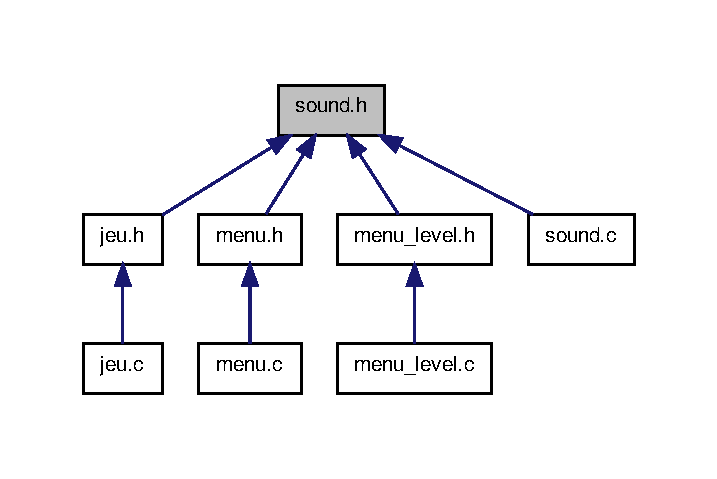
\includegraphics[width=344pt]{sound_8h__dep__incl}
\end{center}
\end{figure}
\subsection*{Data Structures}
\begin{DoxyCompactItemize}
\item 
struct \hyperlink{struct_sound}{Sound}
\end{DoxyCompactItemize}
\subsection*{Functions}
\begin{DoxyCompactItemize}
\item 
\hyperlink{struct_sound}{Sound} $\ast$ \hyperlink{sound_8h_a32a66a56d175c0916741cdf8059091ba}{create\-Sound} (void)
\item 
void \hyperlink{sound_8h_a3af6fda5716d5f42846d0ccc01d5e2ca}{play\-Music} (\hyperlink{struct_sound}{Sound} $\ast$s, char $\ast$file)
\item 
void \hyperlink{sound_8h_a5378cbd0e1d0bfeaa823df1a8ea215f3}{play\-Music\-Once} (\hyperlink{struct_sound}{Sound} $\ast$s, char $\ast$file)
\item 
void \hyperlink{sound_8h_acc13f1ac1e0bac5afe39405869772a08}{free\-Sound} (\hyperlink{struct_sound}{Sound} $\ast$s)
\item 
void \hyperlink{sound_8h_ac3737f55b80ac35471d115d0304e8bc3}{stop\-Sound} (\hyperlink{struct_sound}{Sound} $\ast$s)
\item 
void \hyperlink{sound_8h_a63831c086cacea9358f5c86bebbfb288}{sound\-Volume} (\hyperlink{struct_sound}{Sound} $\ast$s, float volume)
\end{DoxyCompactItemize}


\subsection{Detailed Description}
header de \hyperlink{sound_8c}{sound.\-c} \begin{DoxyAuthor}{Author}
Xavier C\-O\-P\-O\-N\-E\-T 
\end{DoxyAuthor}
\begin{DoxyDate}{Date}
2014-\/02-\/27 
\end{DoxyDate}


\subsection{Function Documentation}
\hypertarget{sound_8h_a32a66a56d175c0916741cdf8059091ba}{\index{sound.\-h@{sound.\-h}!create\-Sound@{create\-Sound}}
\index{create\-Sound@{create\-Sound}!sound.h@{sound.\-h}}
\subsubsection[{create\-Sound}]{\setlength{\rightskip}{0pt plus 5cm}{\bf Sound}$\ast$ create\-Sound (
\begin{DoxyParamCaption}
\item[{void}]{}
\end{DoxyParamCaption}
)}}\label{sound_8h_a32a66a56d175c0916741cdf8059091ba}
créer une structure son \begin{DoxyReturn}{Returns}
la structure son 
\end{DoxyReturn}
\hypertarget{sound_8h_acc13f1ac1e0bac5afe39405869772a08}{\index{sound.\-h@{sound.\-h}!free\-Sound@{free\-Sound}}
\index{free\-Sound@{free\-Sound}!sound.h@{sound.\-h}}
\subsubsection[{free\-Sound}]{\setlength{\rightskip}{0pt plus 5cm}void free\-Sound (
\begin{DoxyParamCaption}
\item[{{\bf Sound} $\ast$}]{s}
\end{DoxyParamCaption}
)}}\label{sound_8h_acc13f1ac1e0bac5afe39405869772a08}
release the sound 
\begin{DoxyParams}[1]{Parameters}
\mbox{\tt out}  & {\em s} & the sound \\
\hline
\end{DoxyParams}
\hypertarget{sound_8h_a3af6fda5716d5f42846d0ccc01d5e2ca}{\index{sound.\-h@{sound.\-h}!play\-Music@{play\-Music}}
\index{play\-Music@{play\-Music}!sound.h@{sound.\-h}}
\subsubsection[{play\-Music}]{\setlength{\rightskip}{0pt plus 5cm}void play\-Music (
\begin{DoxyParamCaption}
\item[{{\bf Sound} $\ast$}]{s, }
\item[{char $\ast$}]{file}
\end{DoxyParamCaption}
)}}\label{sound_8h_a3af6fda5716d5f42846d0ccc01d5e2ca}
lit un fichier long (musique) 
\begin{DoxyParams}[1]{Parameters}
\mbox{\tt in,out}  & {\em s} & la structure son que l'on manipule \\
\hline
\mbox{\tt in}  & {\em file} & Le fichier son à lire \\
\hline
\end{DoxyParams}
\hypertarget{sound_8h_a5378cbd0e1d0bfeaa823df1a8ea215f3}{\index{sound.\-h@{sound.\-h}!play\-Music\-Once@{play\-Music\-Once}}
\index{play\-Music\-Once@{play\-Music\-Once}!sound.h@{sound.\-h}}
\subsubsection[{play\-Music\-Once}]{\setlength{\rightskip}{0pt plus 5cm}void play\-Music\-Once (
\begin{DoxyParamCaption}
\item[{{\bf Sound} $\ast$}]{s, }
\item[{char $\ast$}]{file}
\end{DoxyParamCaption}
)}}\label{sound_8h_a5378cbd0e1d0bfeaa823df1a8ea215f3}
lit un fichier long une fois 
\begin{DoxyParams}[1]{Parameters}
\mbox{\tt in,out}  & {\em s} & la structure son que l'on manipule \\
\hline
\mbox{\tt in}  & {\em file} & Le fichier son à lire \\
\hline
\end{DoxyParams}
\hypertarget{sound_8h_a63831c086cacea9358f5c86bebbfb288}{\index{sound.\-h@{sound.\-h}!sound\-Volume@{sound\-Volume}}
\index{sound\-Volume@{sound\-Volume}!sound.h@{sound.\-h}}
\subsubsection[{sound\-Volume}]{\setlength{\rightskip}{0pt plus 5cm}void sound\-Volume (
\begin{DoxyParamCaption}
\item[{{\bf Sound} $\ast$}]{s, }
\item[{float}]{volume}
\end{DoxyParamCaption}
)}}\label{sound_8h_a63831c086cacea9358f5c86bebbfb288}
set the sound volume 
\begin{DoxyParams}[1]{Parameters}
\mbox{\tt out}  & {\em s} & the sound \\
\hline
\mbox{\tt in}  & {\em volume} & the sound volume \-: \mbox{[}0.\-0 \-: no sound ; 1.\-0 (default) max power\mbox{]} \\
\hline
\end{DoxyParams}
\hypertarget{sound_8h_ac3737f55b80ac35471d115d0304e8bc3}{\index{sound.\-h@{sound.\-h}!stop\-Sound@{stop\-Sound}}
\index{stop\-Sound@{stop\-Sound}!sound.h@{sound.\-h}}
\subsubsection[{stop\-Sound}]{\setlength{\rightskip}{0pt plus 5cm}void stop\-Sound (
\begin{DoxyParamCaption}
\item[{{\bf Sound} $\ast$}]{s}
\end{DoxyParamCaption}
)}}\label{sound_8h_ac3737f55b80ac35471d115d0304e8bc3}
stop the sound 
\begin{DoxyParams}[1]{Parameters}
\mbox{\tt out}  & {\em the} & sound to stop \\
\hline
\end{DoxyParams}

\hypertarget{text_8c}{\subsection{text.\-c File Reference}
\label{text_8c}\index{text.\-c@{text.\-c}}
}


Management of the display of text on the screen.  


{\ttfamily \#include \char`\"{}text.\-h\char`\"{}}\\*
\subsubsection*{Functions}
\begin{DoxyCompactItemize}
\item 
void \hyperlink{text_8c_a1bd80be1aff6fe5303bdd5aa80161da3}{print\-Text} (S\-D\-L\-\_\-\-Surface $\ast$screen, S\-D\-L\-\_\-\-Rect $\ast$pos\-Text, char $\ast$text, int r, int g, int b, char $\ast$font, int pt\-Size, int mode)
\item 
void \hyperlink{text_8c_abd63f9d237bb4bc462d33c00802cd7b9}{capture\-Text} (S\-D\-L\-\_\-\-Surface $\ast$screen, S\-D\-L\-\_\-\-Rect pos\-Text, char $\ast$text, int text\-\_\-length, int r, int g, int b, char $\ast$font, int text\-\_\-size, int $\ast$go)
\end{DoxyCompactItemize}


\subsubsection{Detailed Description}
Management of the display of text on the screen. \begin{DoxyAuthor}{Author}
Xavier C\-O\-P\-O\-N\-E\-T, Glenn H\-E\-R\-R\-O\-U 
\end{DoxyAuthor}
\begin{DoxyDate}{Date}
2014-\/04-\/27 
\end{DoxyDate}


\subsubsection{Function Documentation}
\hypertarget{text_8c_abd63f9d237bb4bc462d33c00802cd7b9}{\index{text.\-c@{text.\-c}!capture\-Text@{capture\-Text}}
\index{capture\-Text@{capture\-Text}!text.c@{text.\-c}}
\paragraph[{capture\-Text}]{\setlength{\rightskip}{0pt plus 5cm}void capture\-Text (
\begin{DoxyParamCaption}
\item[{S\-D\-L\-\_\-\-Surface $\ast$}]{screen, }
\item[{S\-D\-L\-\_\-\-Rect}]{pos\-Text, }
\item[{char $\ast$}]{text, }
\item[{int}]{text\-\_\-length, }
\item[{int}]{r, }
\item[{int}]{g, }
\item[{int}]{b, }
\item[{char $\ast$}]{font, }
\item[{int}]{text\-\_\-size, }
\item[{int $\ast$}]{go}
\end{DoxyParamCaption}
)}}\label{text_8c_abd63f9d237bb4bc462d33c00802cd7b9}
Capture the text corresponding to the keyboard inputs and display it on the screen at the given position 
\begin{DoxyParams}[1]{Parameters}
\mbox{\tt out}  & {\em screen} & The screen of the game \\
\hline
\mbox{\tt in}  & {\em pos\-Text} & The position of the text. If N\-U\-L\-L, the text is centered \\
\hline
\mbox{\tt out}  & {\em text} & The text to display \\
\hline
\mbox{\tt in}  & {\em r} & red value \\
\hline
\mbox{\tt in}  & {\em g} & green value \\
\hline
\mbox{\tt in}  & {\em b} & blue value \\
\hline
\mbox{\tt in}  & {\em text\-\_\-length} & the text length \\
\hline
\mbox{\tt in}  & {\em font} & The path to the font file \\
\hline
\mbox{\tt in}  & {\em text\-\_\-size} & The text size \\
\hline
\mbox{\tt out}  & {\em go} & The main loop validation \\
\hline
\end{DoxyParams}


Here is the call graph for this function\-:\nopagebreak
\begin{figure}[H]
\begin{center}
\leavevmode
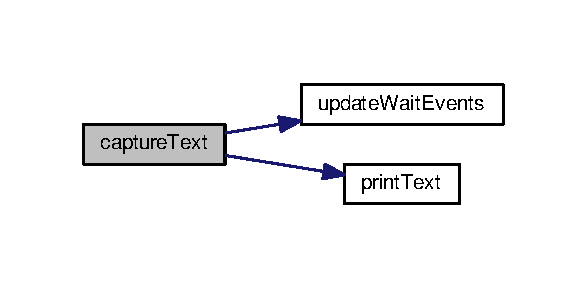
\includegraphics[width=282pt]{text_8c_abd63f9d237bb4bc462d33c00802cd7b9_cgraph}
\end{center}
\end{figure}


\hypertarget{text_8c_a1bd80be1aff6fe5303bdd5aa80161da3}{\index{text.\-c@{text.\-c}!print\-Text@{print\-Text}}
\index{print\-Text@{print\-Text}!text.c@{text.\-c}}
\paragraph[{print\-Text}]{\setlength{\rightskip}{0pt plus 5cm}void print\-Text (
\begin{DoxyParamCaption}
\item[{S\-D\-L\-\_\-\-Surface $\ast$}]{screen, }
\item[{S\-D\-L\-\_\-\-Rect $\ast$}]{pos\-Text, }
\item[{char $\ast$}]{text, }
\item[{int}]{r, }
\item[{int}]{g, }
\item[{int}]{b, }
\item[{char $\ast$}]{font, }
\item[{int}]{pt\-Size, }
\item[{int}]{mode}
\end{DoxyParamCaption}
)}}\label{text_8c_a1bd80be1aff6fe5303bdd5aa80161da3}
Display the given text on the screen, at the given position 
\begin{DoxyParams}[1]{Parameters}
\mbox{\tt out}  & {\em screen} & The screen of the game \\
\hline
\mbox{\tt in}  & {\em pos\-Text} & The position of the text. If N\-U\-L\-L, the text is centered \\
\hline
\mbox{\tt in}  & {\em text} & The text to display \\
\hline
\mbox{\tt in}  & {\em r} & red value \\
\hline
\mbox{\tt in}  & {\em g} & green value \\
\hline
\mbox{\tt in}  & {\em b} & blue value \\
\hline
\mbox{\tt in}  & {\em font} & The path to the font file \\
\hline
\mbox{\tt in}  & {\em pt\-Size} & The text size \\
\hline
\mbox{\tt in}  & {\em mode} & The writing mode \-: 0 (Solid), 1 (Blended) \\
\hline
\end{DoxyParams}

\hypertarget{text_8h}{\subsection{text.\-h File Reference}
\label{text_8h}\index{text.\-h@{text.\-h}}
}


\hyperlink{text_8c}{text.\-c} header  


{\ttfamily \#include $<$stdlib.\-h$>$}\\*
{\ttfamily \#include $<$stdio.\-h$>$}\\*
{\ttfamily \#include $<$errno.\-h$>$}\\*
{\ttfamily \#include \char`\"{}structures.\-h\char`\"{}}\\*
{\ttfamily \#include $<$S\-D\-L/\-S\-D\-L.\-h$>$}\\*
{\ttfamily \#include $<$S\-D\-L/\-S\-D\-L\-\_\-image.\-h$>$}\\*
{\ttfamily \#include $<$S\-D\-L/\-S\-D\-L\-\_\-ttf.\-h$>$}\\*
{\ttfamily \#include \char`\"{}input.\-h\char`\"{}}\\*
\subsubsection*{Functions}
\begin{DoxyCompactItemize}
\item 
void \hyperlink{text_8h_a1bd80be1aff6fe5303bdd5aa80161da3}{print\-Text} (S\-D\-L\-\_\-\-Surface $\ast$screen, S\-D\-L\-\_\-\-Rect $\ast$pos\-Text, char $\ast$text, int r, int g, int b, char $\ast$font, int pt\-Size, int mode)
\item 
void \hyperlink{text_8h_abd63f9d237bb4bc462d33c00802cd7b9}{capture\-Text} (S\-D\-L\-\_\-\-Surface $\ast$screen, S\-D\-L\-\_\-\-Rect pos\-Text, char $\ast$text, int text\-\_\-length, int r, int g, int b, char $\ast$font, int text\-\_\-size, int $\ast$go)
\end{DoxyCompactItemize}


\subsubsection{Detailed Description}
\hyperlink{text_8c}{text.\-c} header \begin{DoxyAuthor}{Author}
Xavier C\-O\-P\-O\-N\-E\-T, Glenn H\-E\-R\-R\-O\-U 
\end{DoxyAuthor}
\begin{DoxyDate}{Date}
2014-\/04-\/27 
\end{DoxyDate}


\subsubsection{Function Documentation}
\hypertarget{text_8h_abd63f9d237bb4bc462d33c00802cd7b9}{\index{text.\-h@{text.\-h}!capture\-Text@{capture\-Text}}
\index{capture\-Text@{capture\-Text}!text.h@{text.\-h}}
\paragraph[{capture\-Text}]{\setlength{\rightskip}{0pt plus 5cm}void capture\-Text (
\begin{DoxyParamCaption}
\item[{S\-D\-L\-\_\-\-Surface $\ast$}]{screen, }
\item[{S\-D\-L\-\_\-\-Rect}]{pos\-Text, }
\item[{char $\ast$}]{text, }
\item[{int}]{text\-\_\-length, }
\item[{int}]{r, }
\item[{int}]{g, }
\item[{int}]{b, }
\item[{char $\ast$}]{font, }
\item[{int}]{text\-\_\-size, }
\item[{int $\ast$}]{go}
\end{DoxyParamCaption}
)}}\label{text_8h_abd63f9d237bb4bc462d33c00802cd7b9}
Capture the text corresponding to the keyboard inputs and display it on the screen at the given position 
\begin{DoxyParams}[1]{Parameters}
\mbox{\tt out}  & {\em screen} & The screen of the game \\
\hline
\mbox{\tt in}  & {\em pos\-Text} & The position of the text. If N\-U\-L\-L, the text is centered \\
\hline
\mbox{\tt out}  & {\em text} & The text to display \\
\hline
\mbox{\tt in}  & {\em r} & red value \\
\hline
\mbox{\tt in}  & {\em g} & green value \\
\hline
\mbox{\tt in}  & {\em b} & blue value \\
\hline
\mbox{\tt in}  & {\em text\-\_\-length} & the text length \\
\hline
\mbox{\tt in}  & {\em font} & The path to the font file \\
\hline
\mbox{\tt in}  & {\em text\-\_\-size} & The text size \\
\hline
\mbox{\tt out}  & {\em go} & The main loop validation \\
\hline
\end{DoxyParams}


Here is the call graph for this function\-:\nopagebreak
\begin{figure}[H]
\begin{center}
\leavevmode
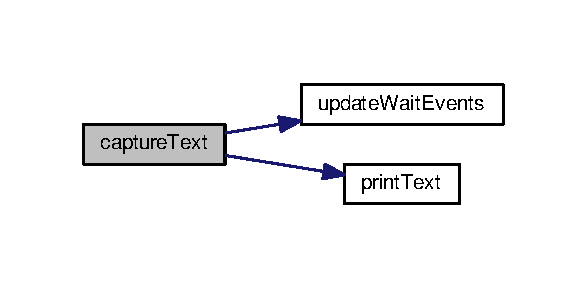
\includegraphics[width=282pt]{text_8h_abd63f9d237bb4bc462d33c00802cd7b9_cgraph}
\end{center}
\end{figure}


\hypertarget{text_8h_a1bd80be1aff6fe5303bdd5aa80161da3}{\index{text.\-h@{text.\-h}!print\-Text@{print\-Text}}
\index{print\-Text@{print\-Text}!text.h@{text.\-h}}
\paragraph[{print\-Text}]{\setlength{\rightskip}{0pt plus 5cm}void print\-Text (
\begin{DoxyParamCaption}
\item[{S\-D\-L\-\_\-\-Surface $\ast$}]{screen, }
\item[{S\-D\-L\-\_\-\-Rect $\ast$}]{pos\-Text, }
\item[{char $\ast$}]{text, }
\item[{int}]{r, }
\item[{int}]{g, }
\item[{int}]{b, }
\item[{char $\ast$}]{font, }
\item[{int}]{pt\-Size, }
\item[{int}]{mode}
\end{DoxyParamCaption}
)}}\label{text_8h_a1bd80be1aff6fe5303bdd5aa80161da3}
Display the given text on the screen, at the given position 
\begin{DoxyParams}[1]{Parameters}
\mbox{\tt out}  & {\em screen} & The screen of the game \\
\hline
\mbox{\tt in}  & {\em pos\-Text} & The position of the text. If N\-U\-L\-L, the text is centered \\
\hline
\mbox{\tt in}  & {\em text} & The text to display \\
\hline
\mbox{\tt in}  & {\em r} & red value \\
\hline
\mbox{\tt in}  & {\em g} & green value \\
\hline
\mbox{\tt in}  & {\em b} & blue value \\
\hline
\mbox{\tt in}  & {\em font} & The path to the font file \\
\hline
\mbox{\tt in}  & {\em pt\-Size} & The text size \\
\hline
\mbox{\tt in}  & {\em mode} & The writing mode \-: 0 (Solid), 1 (Blended) \\
\hline
\end{DoxyParams}

%--- End generated contents ---

% Index
\newpage
\phantomsection
\addcontentsline{toc}{chapter}{Index}
\printindex

\end{document}
